%%%%%%%%%%%%%%%%%%%%%%%%%%%%% EV %%%%%%%%%%%%%%%%%%%%%%%%%%%%%%%%
%
% Trabajo ASS
%
% Autor:  Gema Correa Fernández gecorrea@correo.ugr
%          
%%%%%%%%%%%%%%%%%%%%%%%%%%%%%%%%%%%%%%%%%%%%%%%%%%%%%%%%%%%%%%%%%

\documentclass{manual}

% Includes "References" in the table of contents
\usepackage[nottoc,notlot,notlof]{tocbibind}

% \usepackage{filecontents}
\usepackage[style = ieee, urldate =comp]{biblatex}
\addbibresource{references.bib}

\begin{document}

% Datos del Proyecto %

\newcommand{\authorG}{Correa Fernández, Gema \hspace{0.3cm} 75572158-T \\ \href{mailto:gecorrea@correo.ugr.es}{\textcolor{blue}{\underline{gecorrea@correo.ugr.es}}}}

\title{Certificados Digitales}
\newcommand{\subtitulo}{\textsc{DNI Electrónico}}
\newcommand{\nombrecurso}{Administración de Sistemas y Seguridad}

% Para escribir en color "\textcolor{red}{texto}"
% Para citar: \cite{einstein} (hasta que no se cite no aparece lo de Referencias)

%%%%%%%%%%%%%%%%%%%%%%%%%%%%% PORTADA %%%%%%%%%%%%%%%%%%%%%%%%%%%%%

\begin{titlepage}
  \centering
  %
\includegraphics[height=3cm]{images/!.jpeg}
  %\hfill
  {\textbf{\nombrecurso \vspace*{.1cm}\\} Máster Profesional en Ingeniería Informática \vspace*{.05cm} \\ Universidad de Granada \vspace*{.05cm} \\ Curso académico 2018-2019} \\
  \vspace*{1.5cm}
  
\includegraphics[height=4cm]{images/download-2.png}\\
  \vspace*{2.5cm}
  {\fontsize{28}{34}\selectfont\bfseries \thetitle} \\
  % Línea gris
  \vspace*{0.9cm}
  {\color{gris1}\hrule}
  \Large{\itshape \subtitulo}\\
  \vspace*{3.5cm}
  \begin{center}
    {\large \authorG} \\
  \end{center}
  \vspace{3.5cm}
  
  \textcolor{red}{Toda la información del trabajo se encuentra en: \url{https://github.com/Gecofer/MII_ASS_1819}}
  
  \vspace{0.3cm}
  \begin{center}
      {\large \today}
  \end{center}
\end{titlepage}

%%%%%%%%%%%%%%%%%%%%%%%%%%%%%%%%%%%%%%%%%%%%%%%%%%%%%%%%%%%%%%%%%%%

\newpage
% Sumario %
\tableofcontents
\thispagestyle{empty}

\newpage
\setcounter{page}{1}


% https://www.upv.es/contenidos/CD/info/711545normalc.html
% https://firmaelectronica.gob.es/Home/Ciudadanos/Certificados-Electronicos.html


\section{Certificado digital}

Imaginemos una situación cotidiana: \textit{una persona en un establecimiento desea pagar sus compras con su tarjeta de crédito}. Para ello, dicha persona debe firmar un documento en el que da su conformidad a que se le descuente de su cuenta el importe gastado. Pero, ¿cómo puede estar seguro el responsable del establecimiento de que el qué firma es el propietario de la tarjeta? Normalmente, el responsable pide el \textbf{DNI} a dicha persona, para así comprobar la identidad del firmante. Por tanto, para verificar dicha identidad, se recurre a un documento que asegura que esa persona es quién dice ser. Puesto que en ese documento confiamos, ya que confiamos en la entidad que ha emitido el DNI (Dirección General de Policía, Ministerio del Interior). Es decir, para verificar a la persona ha habido que recurrir a una tercera parte, en quien se confía, y que asegura que la persona no está mintiendo acerca de su identidad.

Si pasamos esto al mundo de las comunicaciones digitales, la situación que se acaba de plantear es muy similar: si alguien firma un documento con una firma digital, ¿cómo puede convencer a quién lo recibe de que la firma la ha realizado esa persona? Se puede comprobar que esa firma se ha realizado con una determinada clave privada, pero ¿corresponde esa clave privada con quién dice realizar la firma? Aquí es donde entra lo que se conoce como una tercera parte de confianza, es decir, algo o alguien en quien confían tanto el firmante como el que recibe la firma. Esa tercera parte de confianza, emite un \textbf{certificado digital} (también llamado certificado electrónico) que no es más que un documento digital en el que se relaciona una identidad con unos datos, y que va firmado digitalmente por quién lo emite.


\subsection{¿Qué es el certificado digital o certificado eléctronico?}

Un \textbf{certificado digital} o \textbf{certificado electrónico} es un documento que identifica a una persona (física o jurídica) con un par de claves. Es expedido por una Autoridad de Certificación, es decir, está firmado electrónicamente por un prestador de servicios de certificación\footnote{Se denomina prestador de servicios de certificación, la persona física o jurídica que expide certificados electrónicos o presta otros servicios en relación con la firma electrónica.}, considerado por otras entidades como una autoridad que vincula unos datos de verificación de firma a un firmante. El certificado digital es el único medio que permite garantizar técnica y legalmente la identidad de una persona en Internet. 

El objetivo de este certificado es validar y certificar que una firma electrónica se corresponde con una persona o entidad concreta, siendo un requisito indispensable para que las instituciones puedan ofrecer servicios seguros a través de la red. Tiene una estructura de datos que contiene información necesaria para firmar electrónicamente e identificar a su firmante con sus datos. Para ello, todo certificado digital debe tener:

\begin{itemize}
	\item Información relativa al propietario del certificado. 
	\item Información relativa al emisor del certificado.
	\item Claves del propietario.
	\item Firma digital del certificado por el emisor.
\end{itemize}

Por tanto, el certificado permite la firma electrónica de documentos: \textit{el receptor de un documento firmado puede tener la seguridad de que éste es el original y no ha sido manipulado y, el autor de la firma electrónica no podrá negar la autoría de esta firma}. Asimismo, la autoridad de certificación da fe de que la firma electrónica se corresponde con un usuario concreto. Además, la firma de la estructura de datos agrupa la información que contiene, de forma que no pueda ser modificada sin que ésta modificación sea detectada.

\subsection{¿Qué son las claves digitales?}

Un certificado digital consta de una pareja de \textbf{claves criptográficas}, es decir, una \textbf{clave pública} y una \textbf{clave privada}, creadas con un algoritmo matemático, esenciales para la firma e identificación del firmante. Ambas claves trabajan de forma complementaria, esto es, lo que cifra o codifica una clave sólo lo puede descifrar o decodificar la otra. La diferencia entre ellas es que la clave privada está pensada para que nunca salga del certificado y esté siempre bajo el control del firmante. En cambio, la clave pública se puede repartir o enviar a otros usuarios o entidades. 

Por esta razón, se puede concluir que la clave pública forma parte de lo que se denomina certificado digital en sí, ya que dicho certificado contiene la clave pública junto con los datos del titular, y firmado electrónicamente por una Autoridad de Certificación. 

Por otra parte, el dueño del certificado debe mantener siempre la clave privada bajo su control, ya que si ésta es sustraída, se podría suplantar la identidad del titular en la red. En este caso, el sujeto debería revocar el certificado lo antes posible, del mismo modo que si anulásemos una tarjeta de crédito.


\subsection{Formato de los certificados digitales}

\begin{figure}[H]
	\centering
	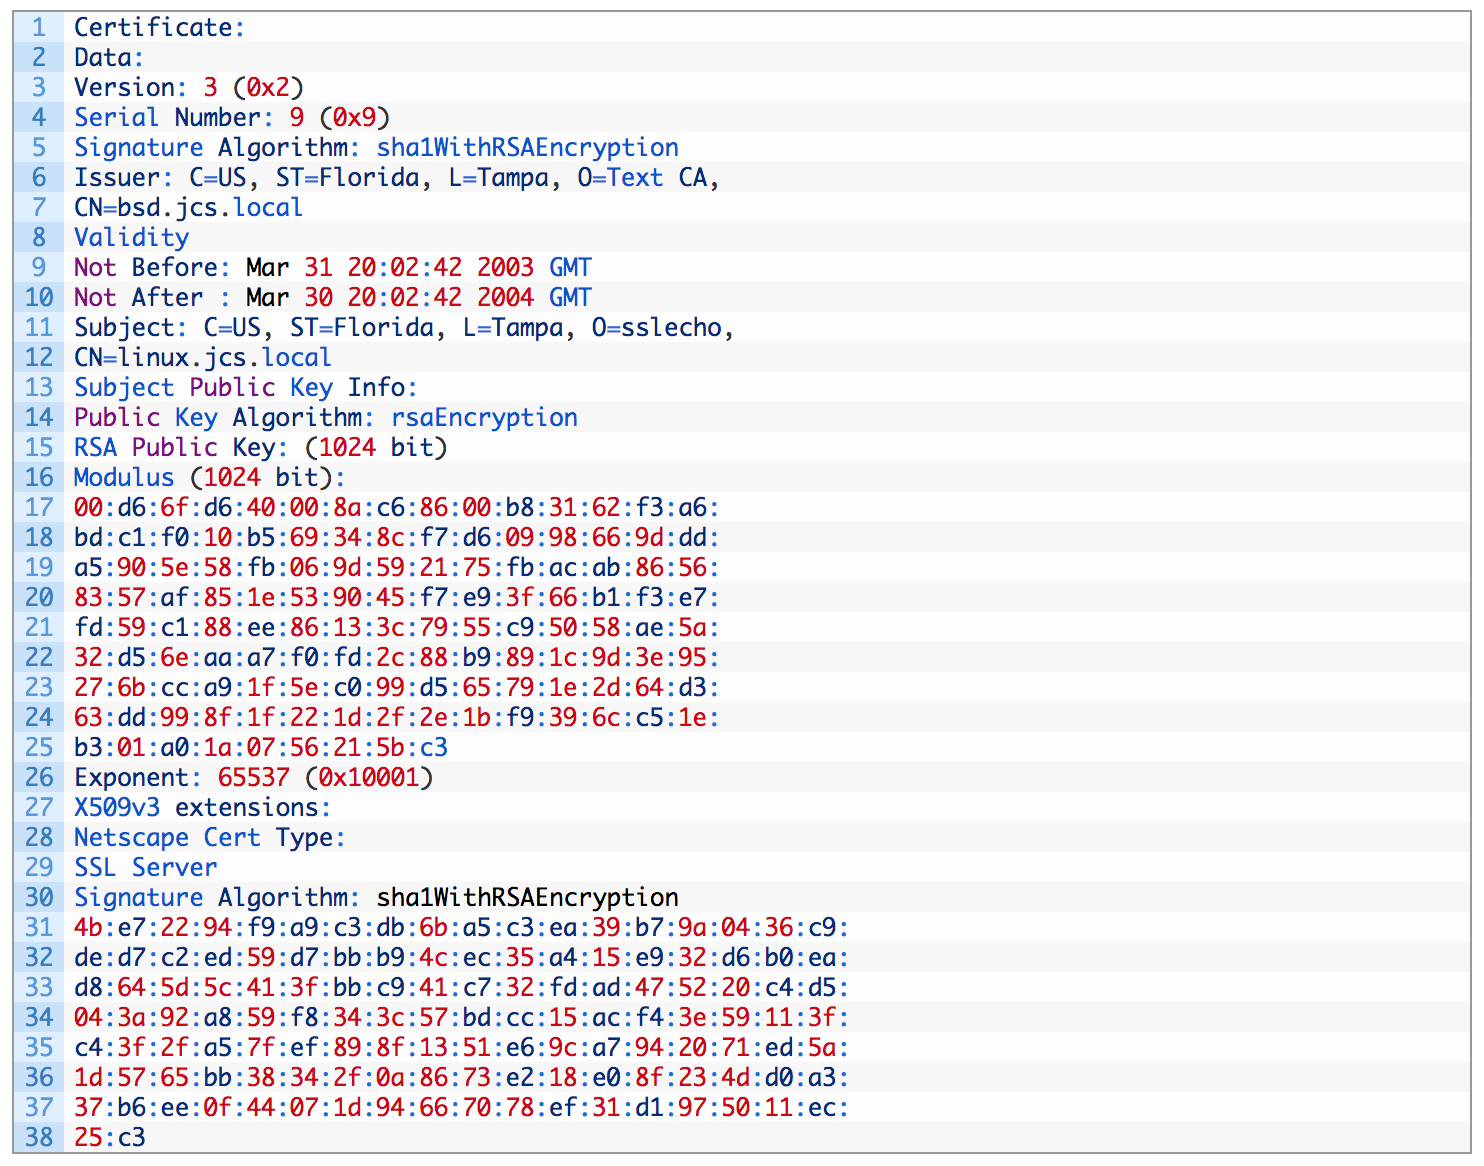
\includegraphics[width=105mm]{images/x509}
	\caption{Ejemplo de un certificado X.509} 
	\label{tipo}
\end{figure}

En la figura \ref{tipo} podemos ver un ejemplo de un certificado X.509. El \textbf{formato X.509} es el más común de los certificados digitales. Es un conjunto estándar de campos con información referente al usuario y al emisor. Está definido por el estándar internacional \textit{ITU-T X.509}, de esta forma, los certificados pueden ser leídos o escritos por cualquier aplicación que cumpla con dicho estándar. Existen 3 versiones de dicho certificado: la primera de 1988, la segunda de 1993 y la tercera de 1996. Los certificados X.509 deben contener los siguientes campos:

\begin{table}[H]
	\begin{tabular}{|m{3.5cm}||m{10cm}|}
		\hline
		\textbf{Versión} &  Especifica la versión del estándar X.509 que se ha empleado (puede ser la 1, la 2 o la 3).\\ \hline
		\textbf{Número de serie}        & Cada vez que una entidad crea un certificado se debe asociar un número de serie, que no puede repetir en otro certificado. \\ \hline
		\textbf{Algoritmo de\newline firma} &  Especifica el algoritmo que ha usado el emisor para firmar el certificado.\\ \hline
		\textbf{Entidad emisora} & Nombre de la entidad que emite el certificado. \\ \hline
		\textbf{Periodo de validez} &  Por seguridad, los certificados tienen un tiempo de vida: se indica cuando comienza a ser válido y cuando dejará de serlo.  \\ \hline
		\textbf{Datos del sujeto} &  Datos identificativos del dueño del certificado.\\ \hline
		\textbf{Clave pública del sujeto} & La clave pública del dueño del certificado, y el algoritmo asociado. \\ \hline
		\textbf{ID único de la \newline entidad emisora} & Una cadena de bits que se usa para identificar a la entidad emisora.  \\ \hline
		\textbf{ID único del \newline sujeto} & Una cadena de bits que se usa para identificar al dueño. \\ \hline
		\textbf{Extensiones} &  Información adicional permitida por el estándar.\\ \hline
		\textbf{Firma digital de la entidad emisora}   & Firma de todos los campos anteriores del certificado, realizada con la clave privada de la entidad emisora.
  \\ \hline
	\end{tabular}
\end{table}


En España la entidad que más certificados digitales ha emitido es la \textbf{Fábrica Nacional de Moneda y Timbre (FNMT)}, a través de la autoridad pública de Certificación Española (CERES). 



% https://www.adminfacil.es/dni-electronico-vs-certificado-digital/
\subsection{Tipos de certificados digitales}

La obtención del certificado digital depende de si el certificado está contenido en una tarjeta, como el DNI-e, o de si el certificado se guarda en un fichero software. No obstante, para ambos casos se debe de identificar al propietario del mismo, lo que requiere que dicha persona se presente en las oficinas de una Autoridad de Registro, para corroborar su identidad. Prácticamente, todas las webs que requieran de certificado funcionan tanto con uno como con otro (ver figura \ref{cita}). 

Entonces, podemos concluir que distinguimos dos tipos de certificados, principalmente:

\begin{enumerate}
	\item El \textbf{certificado contenido en una tarjeta}, como el \textbf{DNI-e} o DNI electrónico, que se incluye en el chip del DNI.
	\item El \textbf{certificado software emitido por la Fábrica Nacional de Moneda y Timbre} (FNMT).
\end{enumerate}

Si se desea obtener el certificado que incluye el DNI electrónico lo único que se necesita es el carnet de identidad, ya que en ese momento se proporciona un sobre con el PIN del DNI-e. Por el contrario, si se decide utilizar los certificados del DNI electrónico se deberá adquirir un lector de tarjetas y renovar los certificados en el tiempo estipulado. Para el caso de los certificados software emitidos por la FNMT, el PIN no será necesario una vez se haya instalado, ya que es el propio navegador del usuario quién crea las claves. %Tiene mayor validez que los certificados que incluye el DNI-e, con lo cual no se deberá de renovar tantas veces.

A partir de estas principales diferencias, podemos destacar las siguientes disimilitudes entre el DNI electrónico y los certificados software.



\begin{table}[H]
	\begin{tabular}{|m{14cm}|}
		\hline
		\textbf{Características del certificado digital} \\ \hline\hline
		La solicitud y descarga del certificado se realizan desde el navegador. Se debe de utilizar el mismo navegador durante todo el proceso, desde la solicitud hasta la descarga final del certificado. \\ \hline
		Se instala en el navegador web en soporte fichero o soporte software, utilizando la extensión .p12 o .pfx.\\ \hline
		Cada proceso de solicitud depende de cada Autoridad de Certificación.\\ \hline
		Sólo funciona en los equipos en los que haya sido instalado, pero existe la posibilidad de exportar los certificados a otros equipos.\\ \hline
		La caducidad de cada certificado depende de la FNMT o de la Autoridad de Certificación, con una media de tres años (36 meses).\\ \hline
	\end{tabular}
\end{table}


\begin{figure}[H]
	\centering
	
\includegraphics[width=25mm]{images/certificado}
	\caption{Mi certificado digital emitido por la FNMT} 
\end{figure}

\begin{figure}[H]
	\centering
	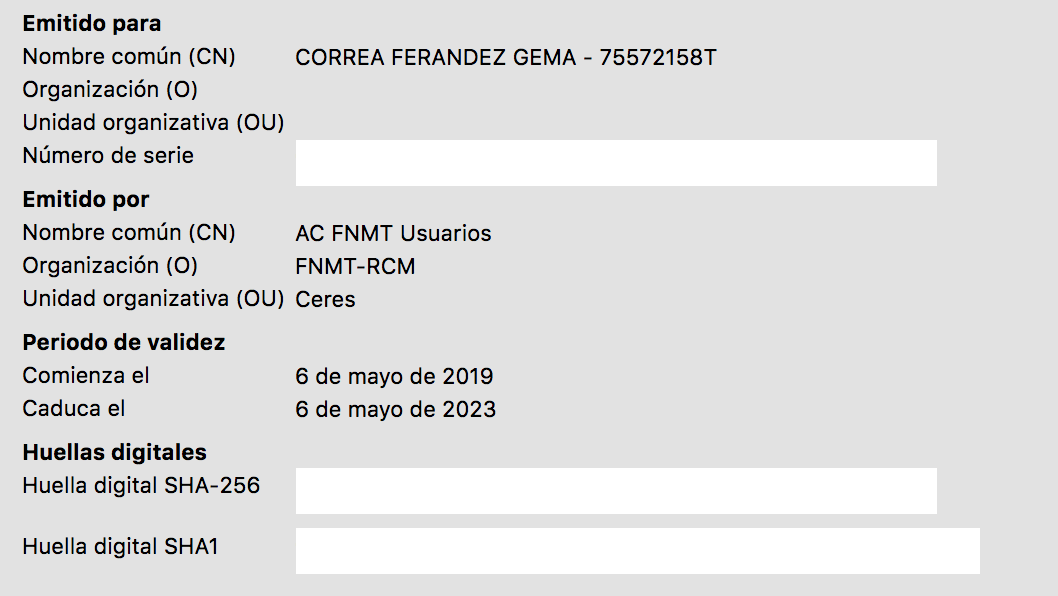
\includegraphics[width=120mm]{images/certificado1}
	\caption{Información acerca de mi certificado digital} 
\end{figure}

\begin{table}[H]
	\begin{tabular}{|m{14cm}|}
		\hline
		\textbf{Características del DNI electrónico} \\ \hline\hline
		Al caducar el Documento Nacional de Identidad, también extinguirán su validez los certificados incorporados en el DNI-e. \\ \hline
		A diferencia del certificado software, la firma electrónica con DNI-e sí es considerada como firma electrónica reconocida, ya que en este caso se trata de un dispositivo de creación de firmas seguro.\\ \hline
		Se necesita un lector de tarjetas en el caso de que se desee utilizar el DNI electrónico, sin embargo, el lector no será necesario, si se posee el nuevo DNI 3.0 ya que incorpora la tecnología NFC.\\ \hline
		Obtener estos certificados es gratis, pero en el caso de renovación o pérdida del DNI-e, se tendrá que pagar un coste.\\ \hline
		Su duración suele ser de 30 meses, y para solicitar uno nuevo deberemos hacerlo presencialmente, con o sin renovación del DNI.\\ \hline
	\end{tabular}
\end{table}

\begin{figure}[H]
	\centering
	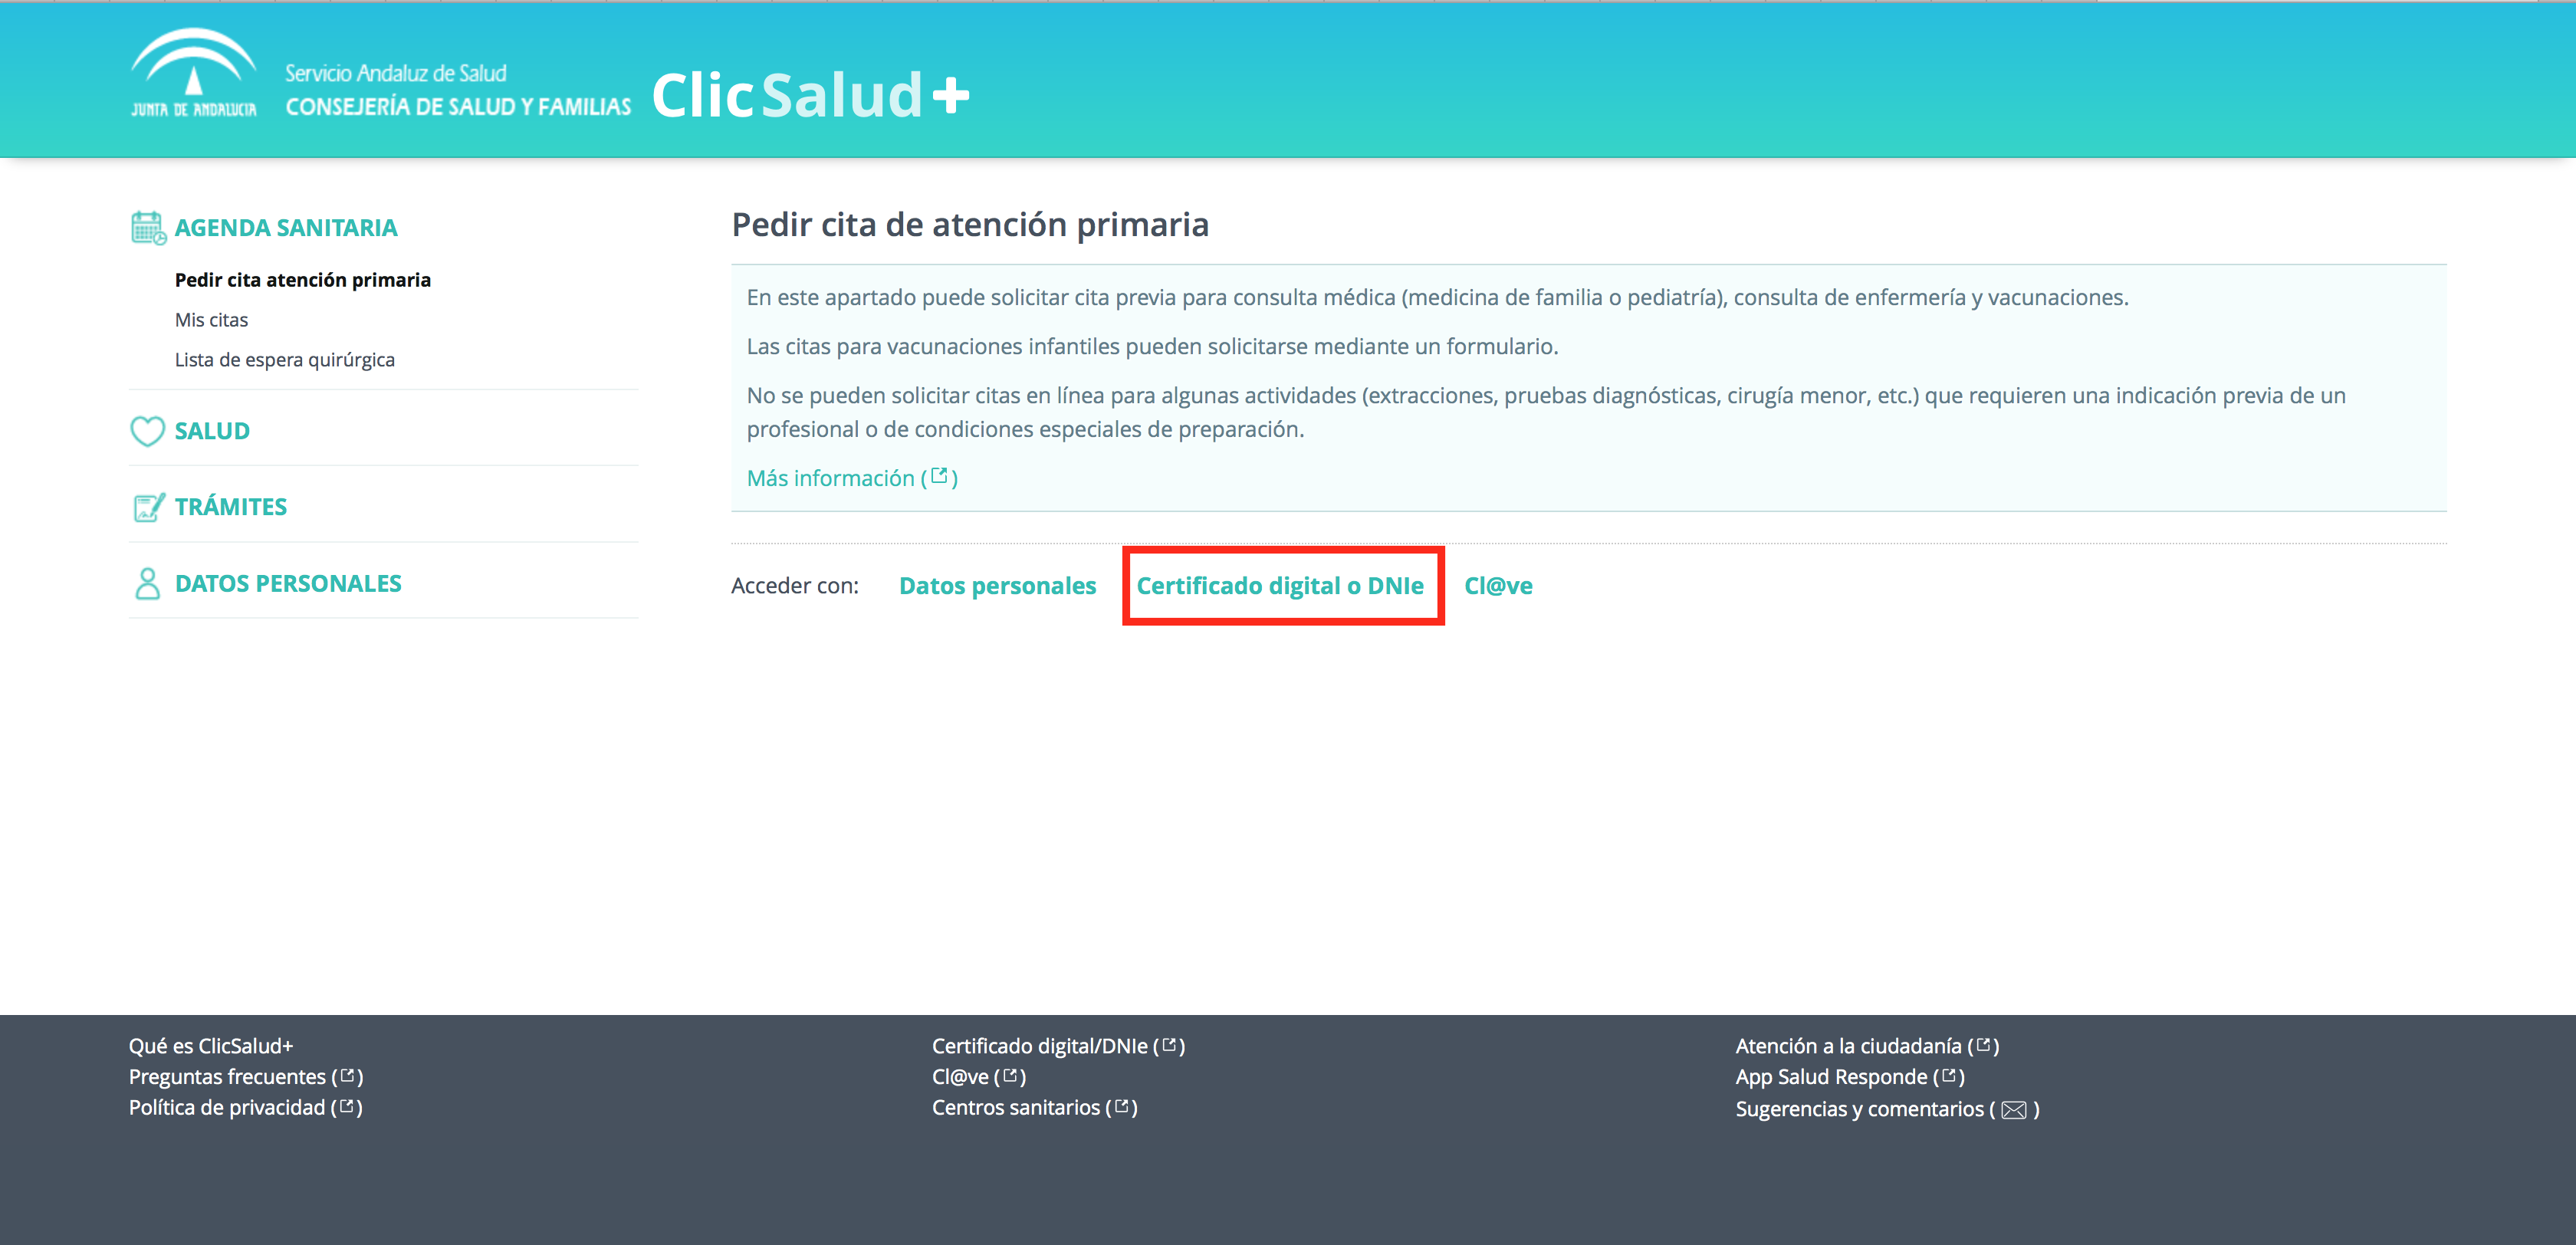
\includegraphics[width=140mm]{images/cita}
	\caption{Pedir cita de atención primaria en el SAS} 
	\label{cita}
\end{figure}

\begin{figure}[H]
	\centering
	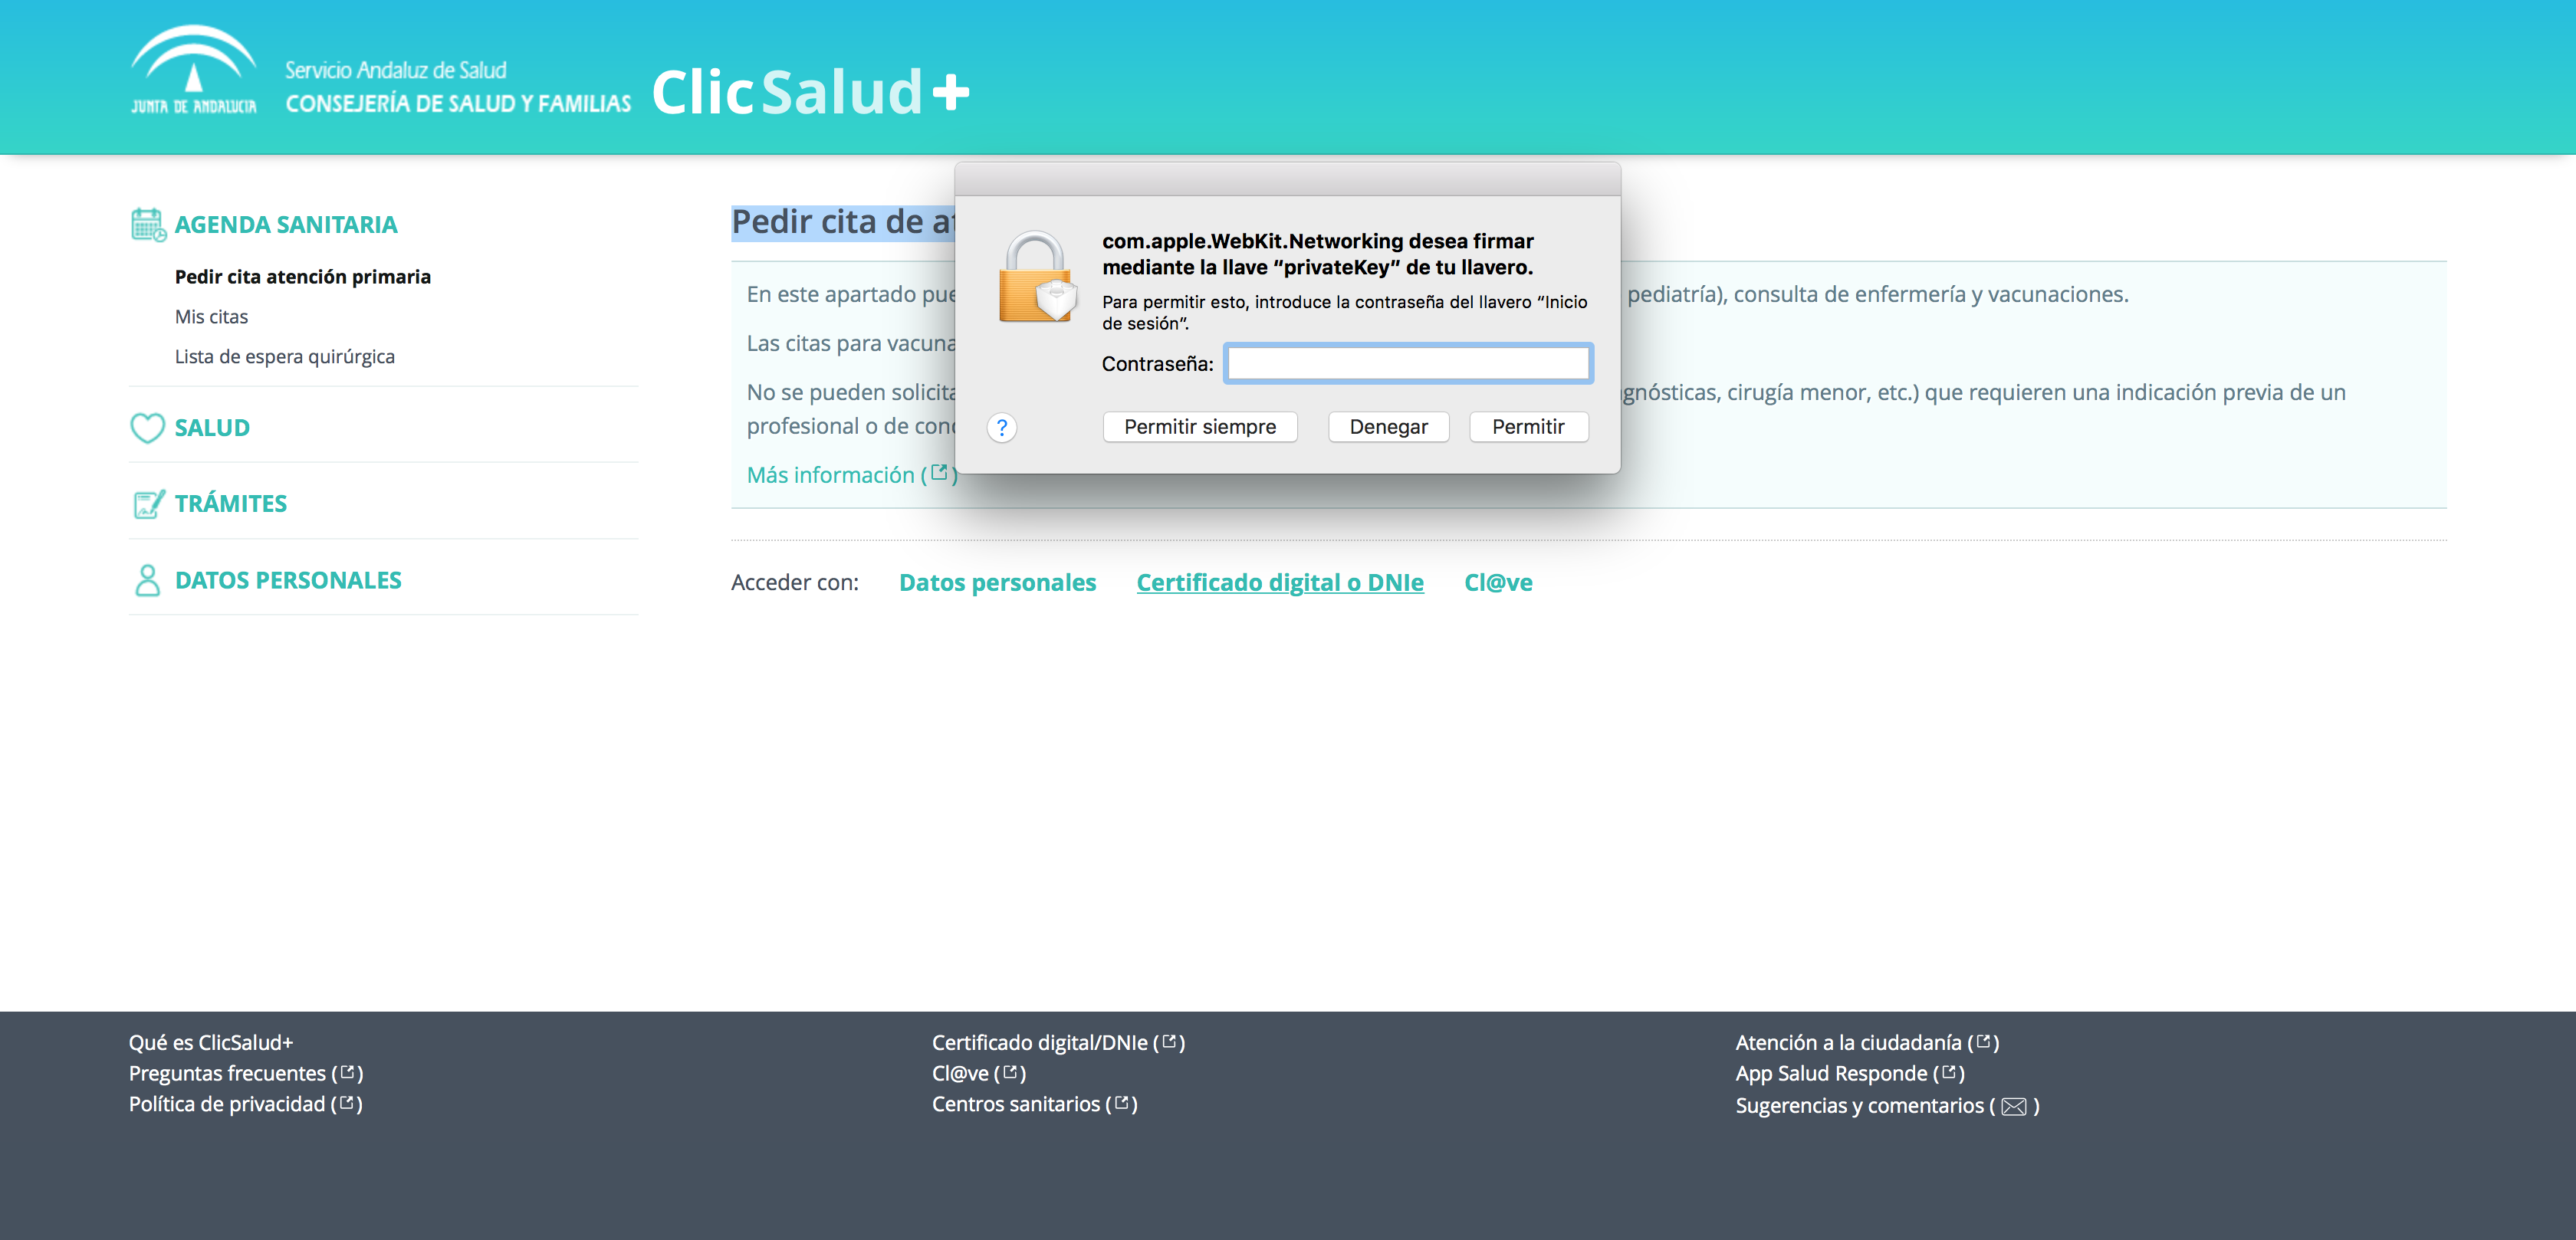
\includegraphics[width=140mm]{images/cita1}
	\caption{Acceso mediante certificado software (introducir contraseña)} 
\end{figure}

\begin{figure}[H]
	\centering
	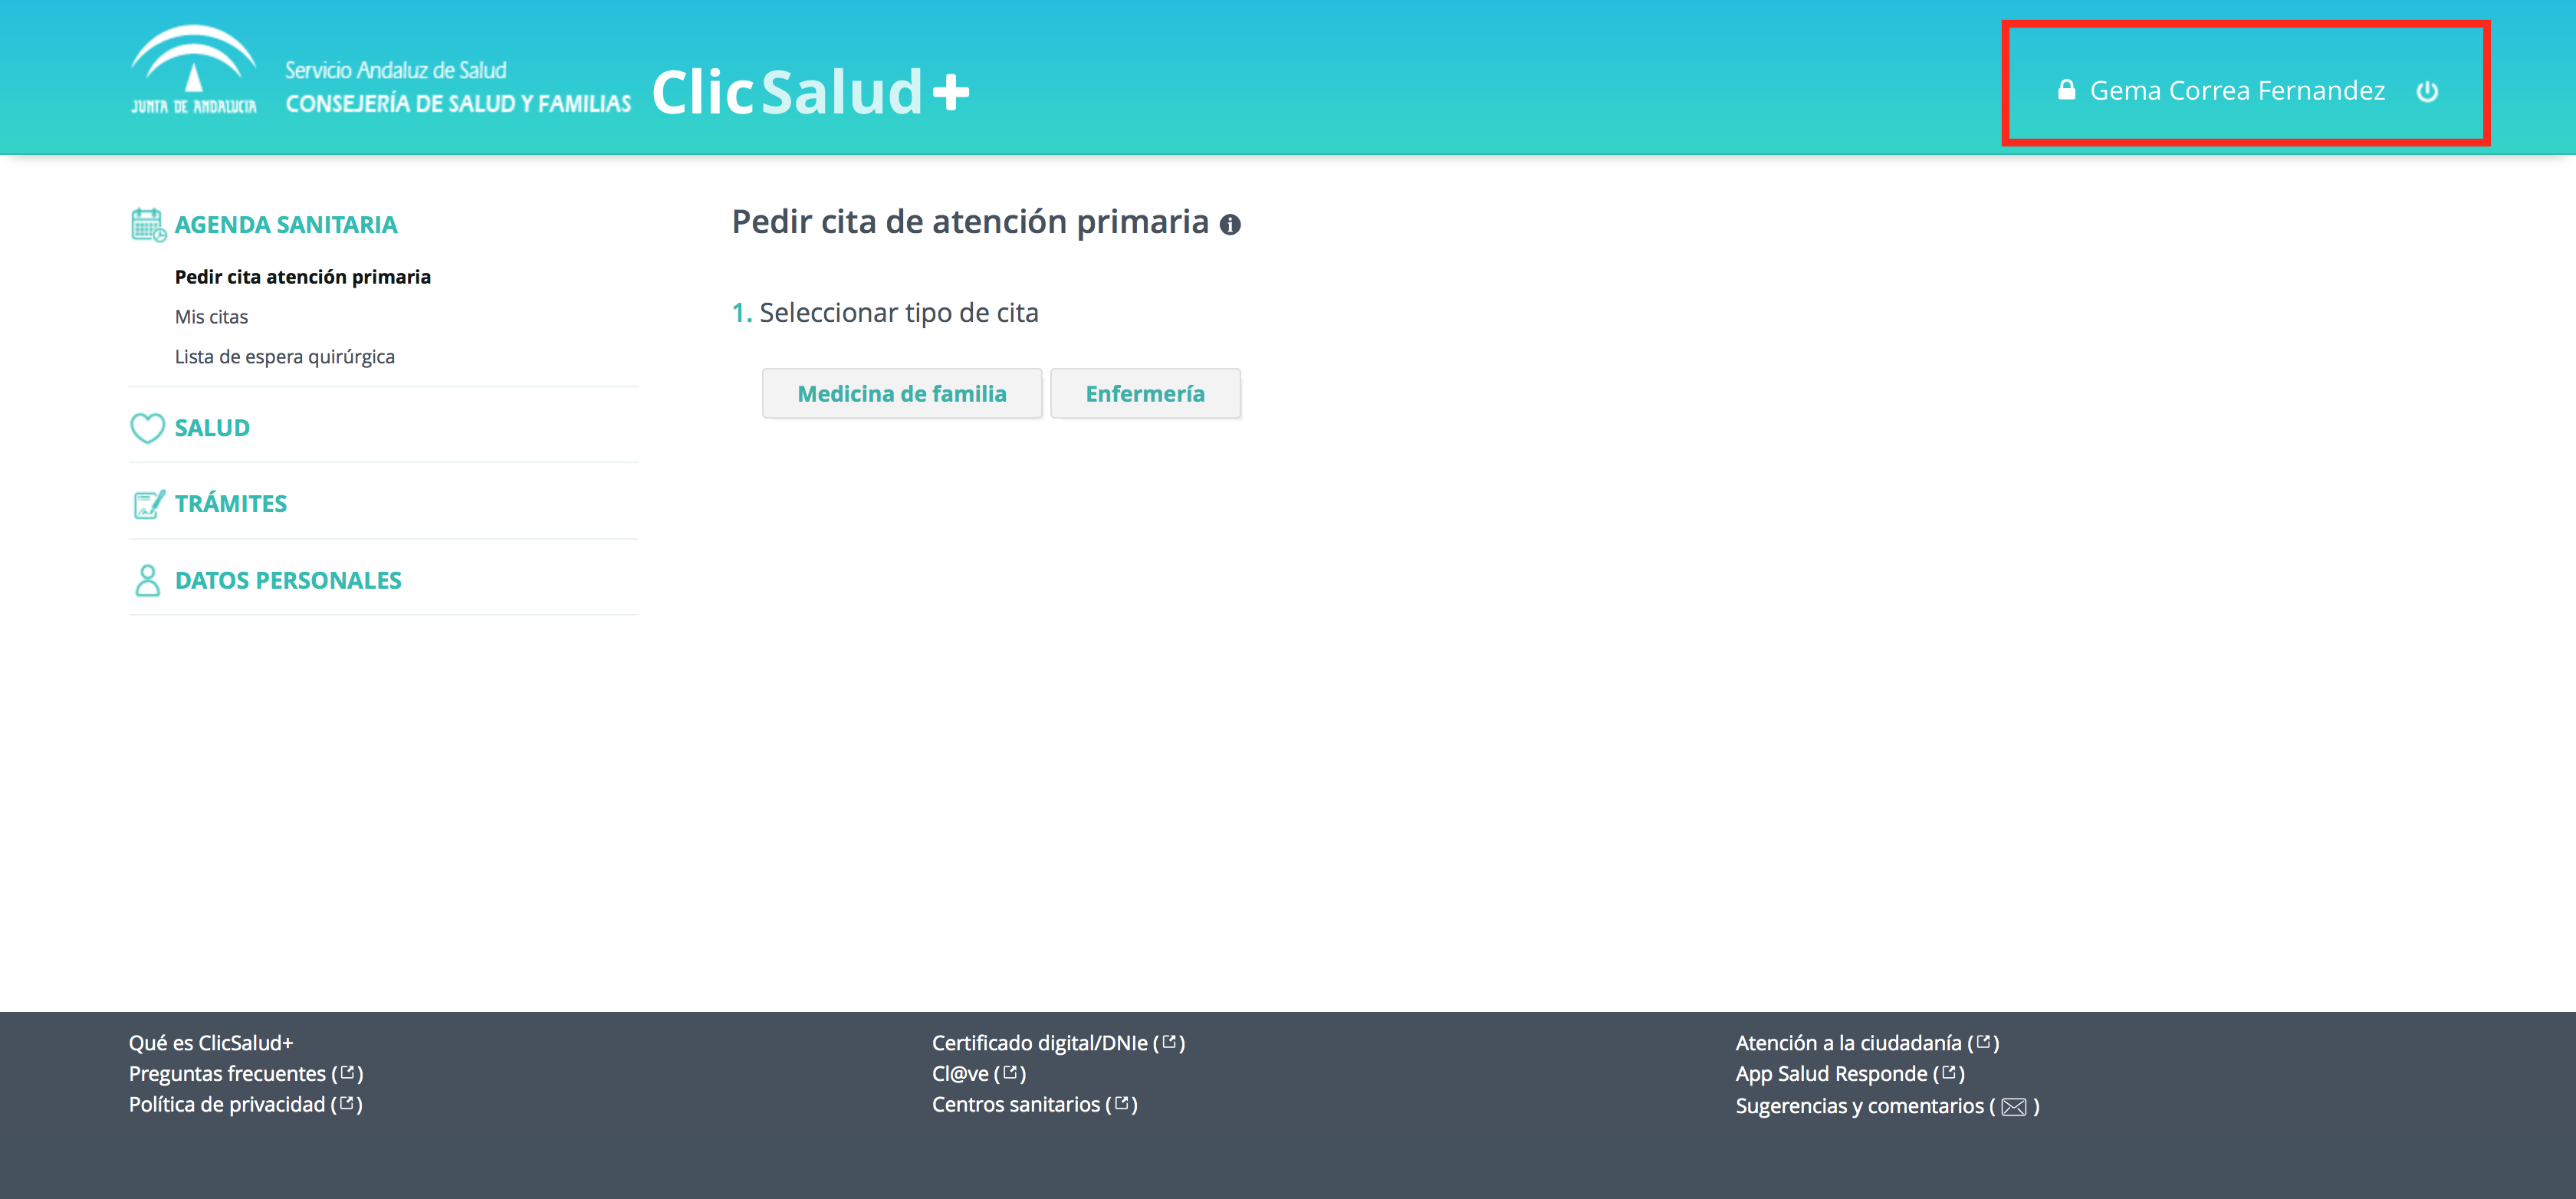
\includegraphics[width=140mm]{images/cita2}
	\caption{Acceso completado} 
\end{figure}


En definitiva, independientemente del certificado que se adquiera, disponer de un certificado permitirá ahorrar tiempo y dinero al realizar trámites administrativos en Internet, a cualquier hora y desde cualquier lugar.


\vspace{0.2cm}
\section{DNI electrónico}

El \textbf{DNI electrónico} es un documento emitido por la Dirección General de la Policía (Ministerio del Interior) y no sólo sirve para confirmar la identidad de una persona concreta, sino para:

\begin{itemize}
	\item Acreditar electrónicamente y de forma inequívoca la identidad de la persona.
	\item Realizar firmas digitales en documentos electrónicos, otorgándoles de la misma validez jurídica que con la firma tradicional.
\end{itemize}

\begin{figure}[H]
	\centering
	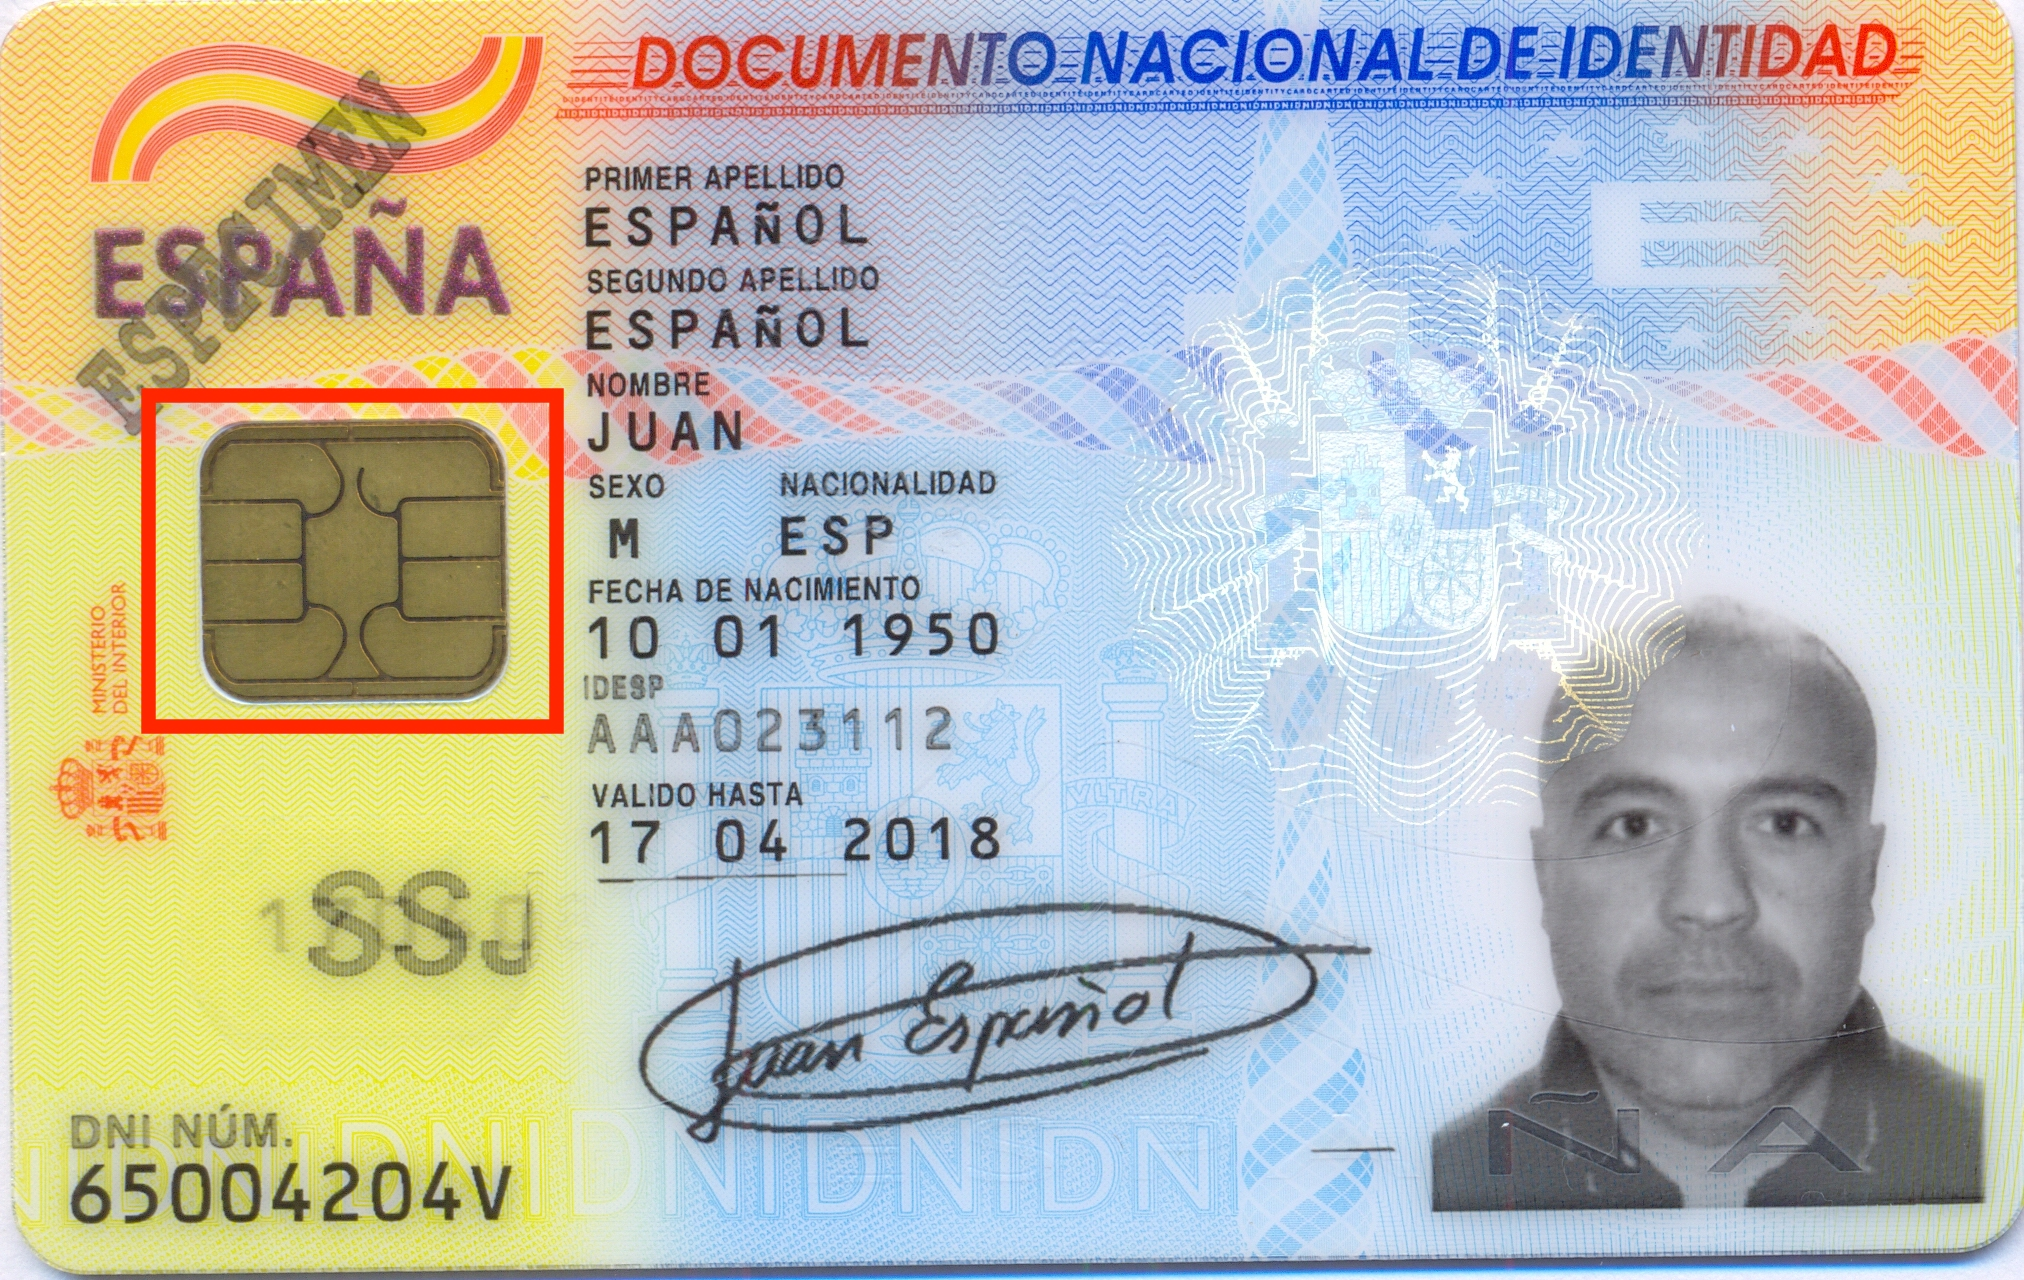
\includegraphics[width=85mm]{images/anverso_2}
	\caption{DNI electrónico} 
	\label{1}
\end{figure}

Adicionalmente, el DNI-e incorpora un pequeño \textbf{circuito integrado} (chip), que contiene los mismos datos que aparecen impresos en la tarjeta (datos personales, fotografía, firma y huella dactilar digitalizada) junto con los certificados de Autenticación y de Firma Electrónica. La importancia del certificado en el DNI electrónico reside en el chip que contiene (ver figura \ref{1}), gracias a él, podemos obtener los certificados:




\begin{itemize}
	\item \textbf{Certificado de Autenticación:} tiene como finalidad garantizar electrónicamente la identidad del ciudadano al realizar una transacción telemática, asegurando que la comunicación electrónica se realiza con la persona que dice que es. Así, el titular podrá a través de su certificado acreditar su identidad frente a cualquiera ya que se encuentra en posesión del certificado de identidad y de la clave privada asociada al mismo.
		
	\item \textbf{Certificado de Firma:} tiene como finalidad permitir al ciudadano firmar trámites o documentos. Permite sustituir la firma tradicional por la electrónica en las relaciones del ciudadano con terceros.
\end{itemize}
	

De esta forma, cualquier persona podrá realizar múltiples gestiones online de forma segura con las Administraciones Públicas, con empresas públicas y/o privadas, y con otros ciudadanos, a cualquier hora y sin tener que desplazarse ni hacer colas.


\subsection{Componentes del DNI electrónico}

\begin{figure}[H]
	\centering
	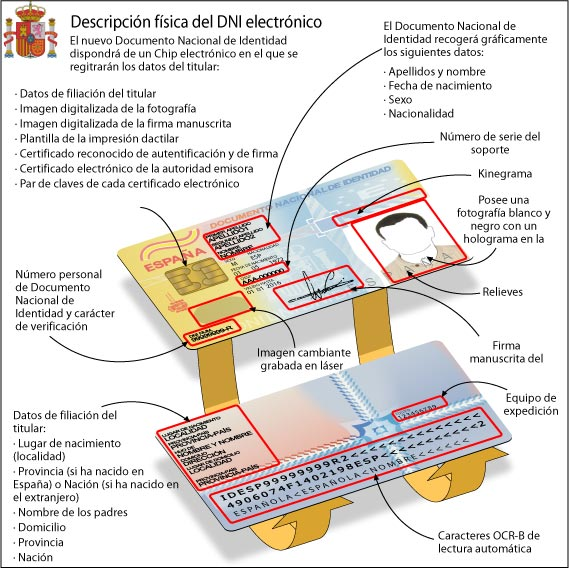
\includegraphics[width=120mm]{images/dnie_descrip}
	\caption{Descripción física del DNI-e} 
	\label{componentes}
\end{figure}

Como bien sabemos, el DNI electrónico es una tarjeta de plástico, que incorpora un chip con información digital y que tiene unas dimensiones idénticas a las del DNI tradicional (85,60 mm de ancho X 53,98 mm de alto). En la figura \ref{componentes}, se observan sus principales componentes. Su validez es de 30 meses (menos de 3 años), siendo renovables por el ciudadano en una oficina de expedición. Se utiliza para firmar electrónicamente SHA-1 y usa claves RSA. 

\subsubsection{Chip criptográfico}

El chip del DNI está localizado en la parte central izquierda del anverso del Documento de Identidad Nacional. Este chip permite dotarlo de la capacidad de ser leído de forma rápida y sencilla por las máquinas, no por las personas. Como se ha comentado, incorpora parte de los mismos datos que aparecen impresos en la tarjeta:

\begin{table}[H]
	\centering
	\begin{tabular}{|c|}
		\hline
		Datos de filiación del titular\\ \hline
		Imagen digitalizada de la fotografía\\ \hline
		Imagen digitalizada de la firma manuscrita\\ \hline
		Plantilla de impresión dactilar\\ \hline
		Certificado reconocido de autenticación y firma\\ \hline
		Certificado electrónico de la autoridad emisora\\ \hline
		Par de claves de cada certificado electrónico\\ \hline
	\end{tabular}
\end{table}

Respecto a las características del chip, mencionar que contiene el sistema operativo DNIe v1.1 con una capacidad de información de 32KB. Además, dicha información está clasificada en zonas diferentes según su accesibilidad:

\begin{itemize}

	\item \textbf{Zona pública}, accesible en lectura sin restricciones, contiene la Autoridad de Certificación, que es la entidad responsable de emitir el certificado, claves \textit{Diffie-Hellman}, que es un protocolo criptográfico para compartir claves y formato X.509 para el certificado (\textit{visto anteriormente}).
	
		
	\item \textbf{Zona privada}, accesible en lectura por el ciudadano mediante una Clave Personal de Acceso o PIN, y contiene los Certificados de Autenticación y de Firma.
		
		%\begin{itemize}
		%	\item Certificado de Firma (para firmar documentos, garantiza integridad y no repudio).
		%	\item Certificado de Autenticación (garantiza electrónicamente la identidad del ciudadano). 
		%\end{itemize}
		
	\item \textbf{Zona de seguridad}, accesible en lectura por el ciudadano en los puntos de actualización del DNI. Contiene los datos de filiación del ciudadano contenidos en el soporte físico del DNI, la imagen de la fotografía digitalizada y la imagen de la firma manuscrita (digitalizada).
		
\end{itemize}

En lo referente a la estructura de la clave pública para el DNI, se asignan las funciones de Autoridad de Validación y Autoridad de Certificación a entidades diferentes, con el fin de aislar la comprobación de la vigencia de un certificado electrónico de los datos de identidad del titular. Así, la Autoridad de Certificación (Dirección General de la Policía) no puede acceder a los datos de las transacciones que se realicen con los certificados que emite. Y las Autoridades de Validación no tienen acceso a la identidad de los titulares de los certificados electrónico que maneja.



\subsection{Seguridad en el DNI electrónico}

% https://www.dnielectronico.es/PortalDNIe/PRF1_Cons02.action?pag=REF_2100&id_menu=[6]

% https://www.xataka.com/seguridad/la-seguridad-del-dni-electronico-comprometida-a-quien-afecta-por-que-y-como-solucionarlo

% https://www.abc.es/tecnologia/abci-activada-nuevo-firma-digital-tras-alerta-fallos-seguridad-201712011500_noticia.html

% https://elpais.com/politica/2017/11/09/actualidad/1510217634_470836.html

% https://www.ideal.es/sociedad/problema-dni-electronico-afecta-espanoles-20180314093937-nt.html

Uno de los principales usos del DNI-e es la realización de la firma electrónica. Para poder utilizar esta funcionalidad,
es indispensable disponer de funciones de seguridad:

\begin{enumerate}
	\item \textbf{Autenticación}: se dispone de distintos métodos de autenticación, mediante los cuales una entidad externa demuestra su identidad, o el conocimiento de algún dato secreto almacenado en la tarjeta. Entre los distintos tipos de autenticación podemos destacar: \textit{autenticación de usuario (PIN)}, \textit{autenticación de usuarios mediante datos biométricos}, \textit{autenticación de aplicación} y \textit{autenticación mutua}.
	
	\item \textbf{Securización de mensajes}: se permite la posibilidad de establecer un canal seguro entre el terminal y la tarjeta que securice los mensajes transmitidos. Durante la presencia del canal seguro los mensajes se cifran y autentican, de tal forma que se asegura una comunicación \textit{una a uno} entre los dos puntos del canal.	
	
	\item \textbf{Desbloqueo y cambio de PIN}: se permite el cambio de PIN. Debido a la criticidad de esta operación, el cambio de PIN se ha de realizar siempre en condiciones de máxima confidencialidad y seguridad.
	
	\item \textbf{Funcionalidad criptográfica}: 
	
	\begin{itemize}
		\item \textit{Claves RSA}: genera y gestiona claves RSA. Se usa el algoritmo Miller-Rabin como test de primalidad.
		
		\item \textit{Hash}: realiza hash de datos con el algoritmo SHA1. Es posible realizar todo el proceso en la tarjeta o finalizar un hash calculado externamente. 
		
		\item \textit{Firmas electrónicas}: puede realizar firmas electrónicas de distintos modos.
	\end{itemize}

	\item \textbf{Intercambio de claves}: esta operación es usada para compartir claves simétricas entre dos entidades. Es posible cifrar una clave $Ks$ con la clave pública de un destinatario, la cual puede ser cargada en la memoria de la tarjeta protegida mediante una clave RSA. Y el destinatario puede descifrar la clave $Ks$ usando la clave privada RSA correspondiente.
\end{enumerate}	

Sin embargo, el uso de las funciones de seguridad no determina que se puedan encontrar vulnerabilidades en el DNI-e, por ejemplo \textit{en 2017 la Policía desactivó la firma digital del DNI ante un posible fallo de seguridad en el sistema de identificación online, que permitía hacer diversos trámites administrativos, mercantiles y privados. Debido a este problema un atacante podría calcular la porción privada de una clave vulnerable usando tan solo la parte pública. Eso daría lugar a que un atacante acabara pudiendo suplantar la personalidad de la víctima para descifrar datos sensibles, ocultar software malicioso en software firmado digitalmente o superar la protección basada en estos sistemas} (para más información, pincha \href{https://elpais.com/politica/2017/11/09/actualidad/1510217634_470836.html}{\underline{aquí}}).




\subsection{¿Que ventajas nos ofrece el DNI electrónico?}

% https://www.dnielectronico.es/PortalDNIe/PRF1_Cons02.action?pag=REF_230&id_menu=[6]

Gracias al DNI eléctronico, cualquier persona puede realizar múltiples gestiones online de forma segura con distintas personas y/o entidades, sin embargo, esas no son todas las ventajas que ofrece:

\begin{itemize}
	\item \textbf{Respecto a las relaciones entre ciudadanos}: la firma electrónica del DNI-e permite garantizar la identidad de la persona que realiza una gestión, así como la integridad del contenido de los mensajes que envía. Por tanto, los ciudadanos podrán consultar datos de carácter personal, realizar trámites u otras gestiones o acceder a diferentes servicios públicos y privados. Además, proporciona el máximo grado de confidencialidad y seguridad en Internet, identifica a las partes que se conectan telemáticamente y permite el acceso seguro a servicios de Administración Electrónica desde dispositivos móviles.
	
	\item \textbf{Respecto a las relaciones con las Administraciones Públicas}: la Administración General del Estado es uno de los principales proveedores de servicios a utilizar con el DNI electrónico, de esta forma su utilización supone una ventaja en los trámites con la Administración Pública, en la que ya no es necesario la presencia física para garantizar la identidad.
	
	\item \textbf{Respecto a las relaciones con las empresas}: las empresas deben desarrollar diferentes servicios basados en la identificación y firma electrónica, de forma que dinamicen la relación comercial con sus clientes. Por eso, desde el punto de vista empresarial y comercial, el DNI electrónico pasa a convertirse en una herramienta fundamental para las relaciones en el sector privado.
\end{itemize}


\subsection{¿Cómo utilizar el DNI electrónico?}

%Cómo activar los certificados de tu DNI electrónico

% https://computerhoy.com/paso-a-paso/internet/como-activar-certificados-tu-dni-electronico-17513

%donde hay puntos de actualización del dni electrónico

\begin{figure}[H]
	\centering
	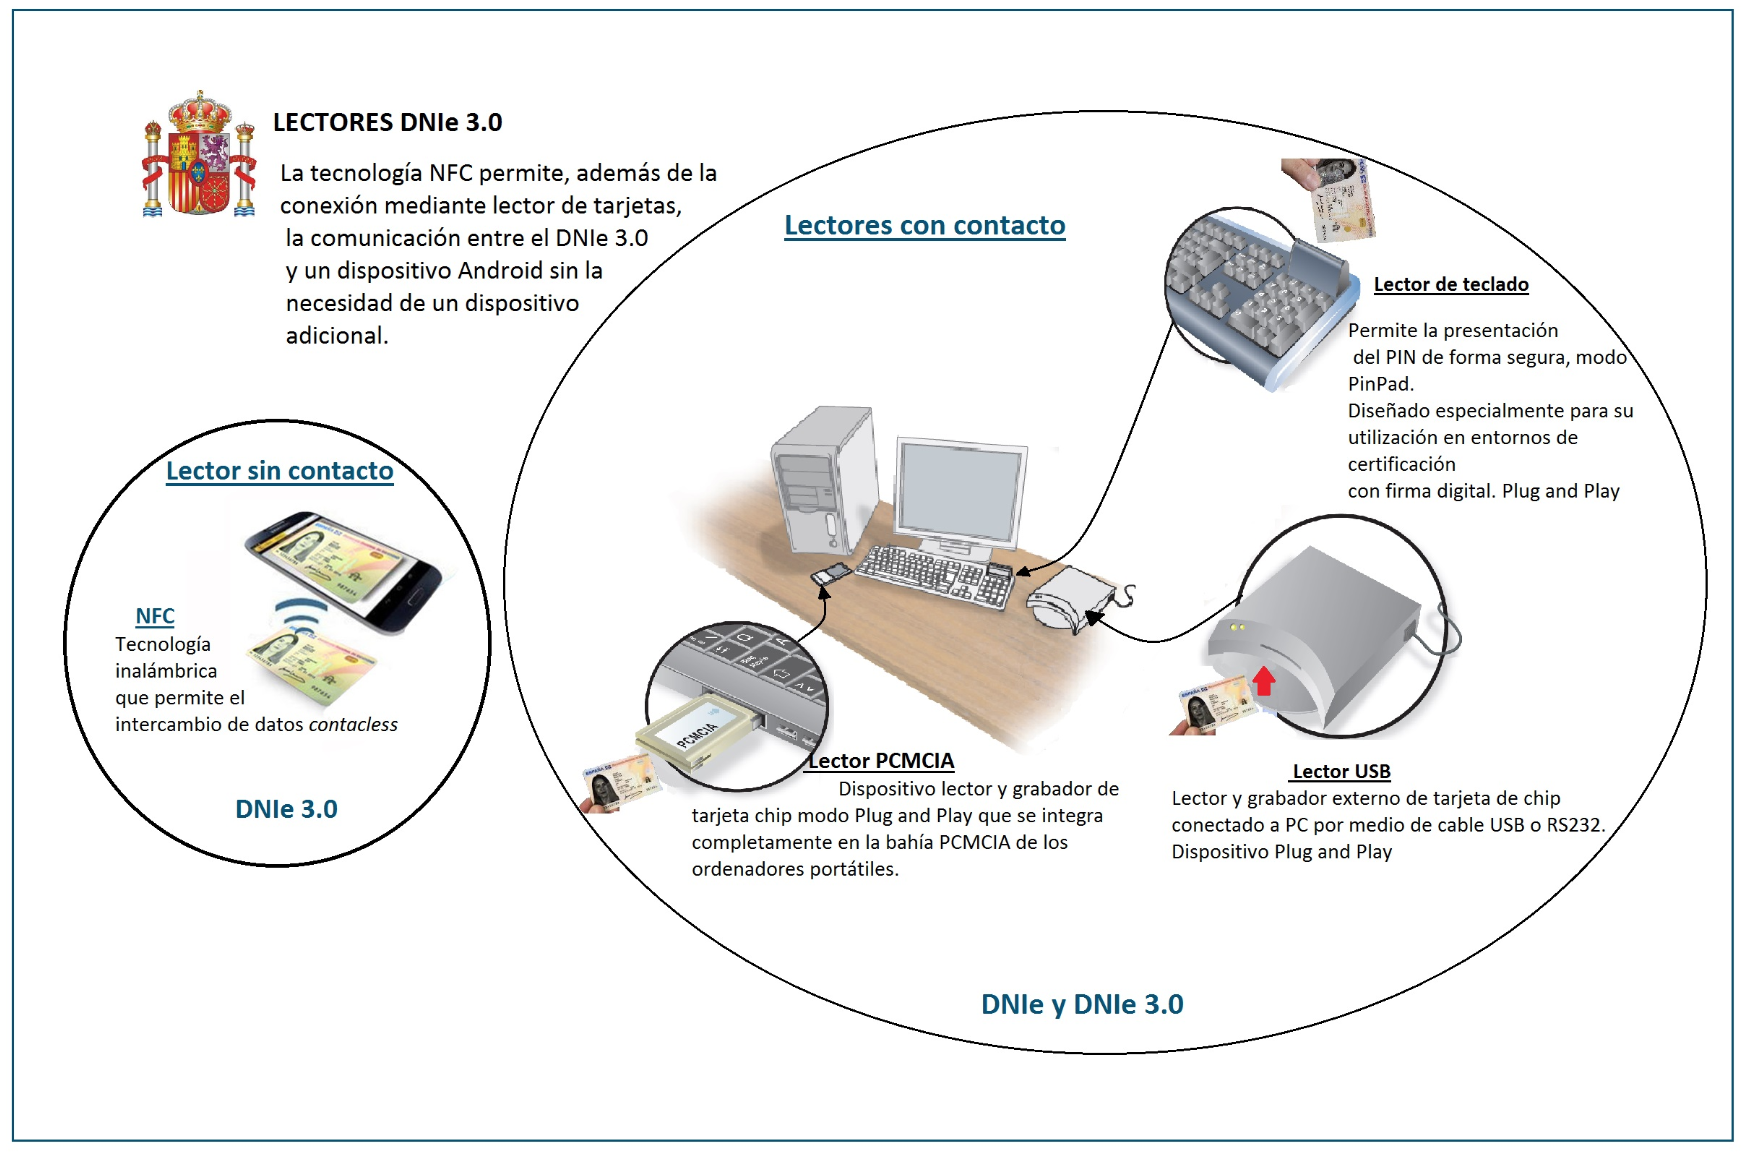
\includegraphics[width=135mm]{images/lectura}
	\caption{Utilización del DNI-e} 
\end{figure}

Para hacer uso del certificado que incluye el DNI electrónico lo único que se necesita es el carnet de identidad, ya que en ese momento se proporciona un sobre con el PIN del DNI-e. Por el contrario, si se decide utilizar los certificados del DNI electrónico se deberá adquirir un lector de tarjetas y renovar los certificados en el tiempo estipulado. Asimismo, para firmar con el DNI-e se necesita:

\begin{itemize}
	\item Un ordenador personal.
	\item Un lector de tarjetas inteligentes. %Existen distintas implementaciones, bien integrados en el teclado, bien externos (conectados vía USB) o bien a través de una tarjeta PCMCIA.
	\item En cuanto a software, el DNI electrónico es compatible con los sistemas operativos actuales, así como con los distintos navegadores. 
\end{itemize}



%Los requisitos Técnicos: Controladores / Módulos Criptográficos Para poder interaccionar adecuadamente con las tarjetas criptográficas y con el DNI electrónico, tu equipo ha de tener instalados unas ‘piezas’ de software denominadas módulos criptográficos. En un entorno Microsoft Windows, el equipo debe tener instalado un servicio que se denomina "CryptographicServiceProvider" (CSP). En los entornos UNIX / Linux o MAC es posible utilizar el DNI-e a través de un módulo criptográfico denominado PKCS\#11.



\subsection{Diferencias entre DNI-e y DNI 3.0}

% https://www.dnielectronico.es/PortalDNIe/PRF1_Cons02.action?pag=REF_038

Los cambios en la sociedad de hoy en día requieren de la constante actualización del DNI, esto ha supuesto la necesidad de mejorar y acercar a los ciudadanos su usabilidad. Por lo que la Dirección General de la Policía lanzó en 2015 el \textbf{DNI 3.0}. Sin embargo, tenemos que irnos hasta el año 2006 para presenciar que todos los Documentos Nacionales de Identidad que se expedían en España comienzan a ser documentos electrónicos. 

Hoy en día, existen dos versiones: DNI-e y DNI 3.0, aunque el único documento que se expide actualmente es en el DNI 3.0. Hasta ahora hemos visto que el uso del DNI electrónico requiere de un dispositivo para la lectura de los datos del chip, así como la necesidad de la instalación de drivers necesarios para el funcionamiento del hardware, cosa que puede resultar complicada para un usuario normal.

\begin{figure}[H]
	\centering
	\subfigure[DNI-e]{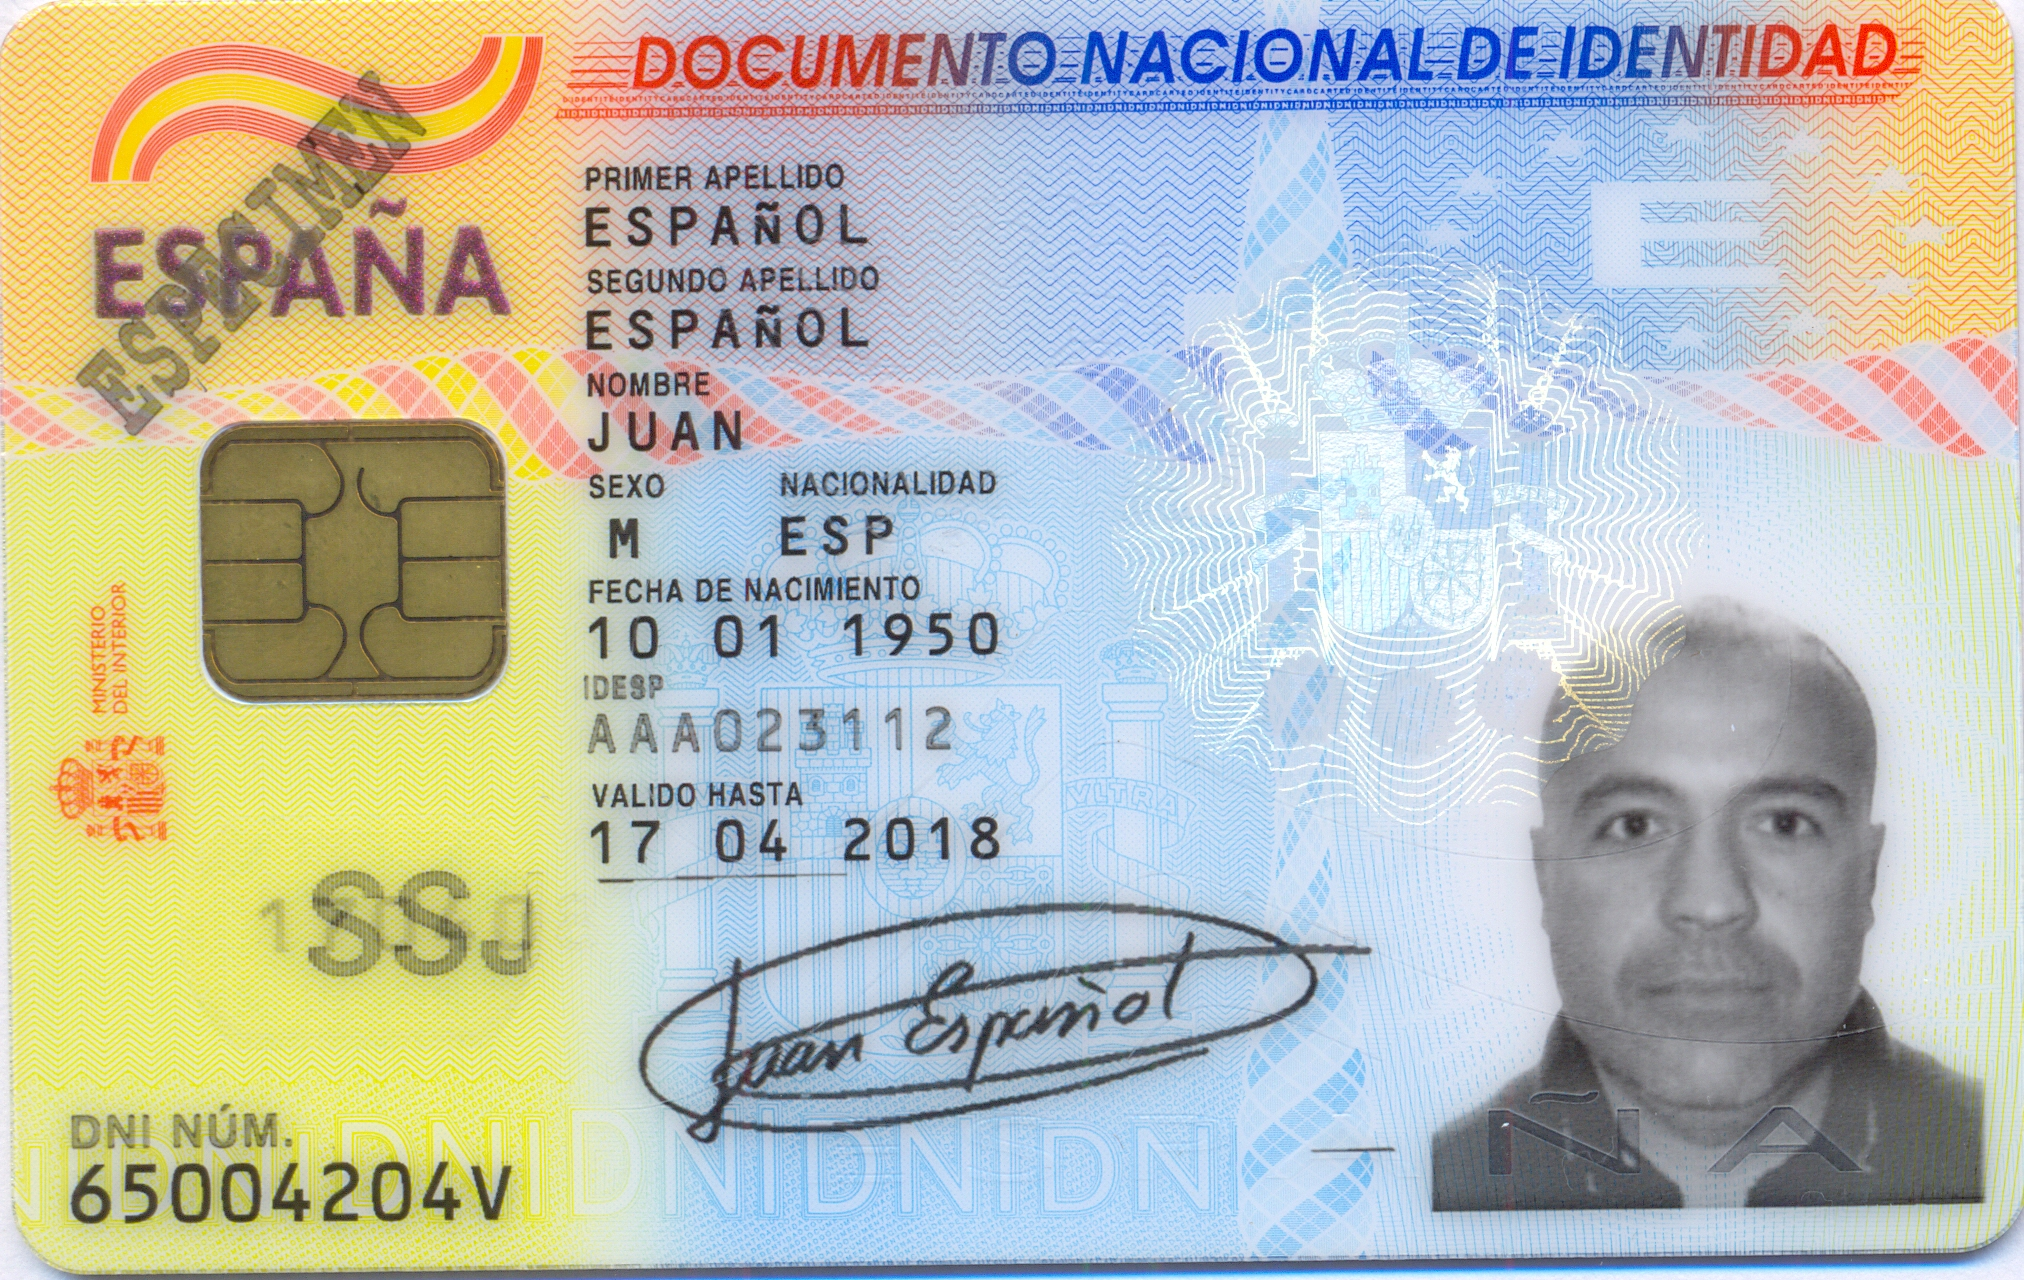
\includegraphics[width=65mm]{images/anverso_4.jpg}}
	\subfigure[DNI 3.0]{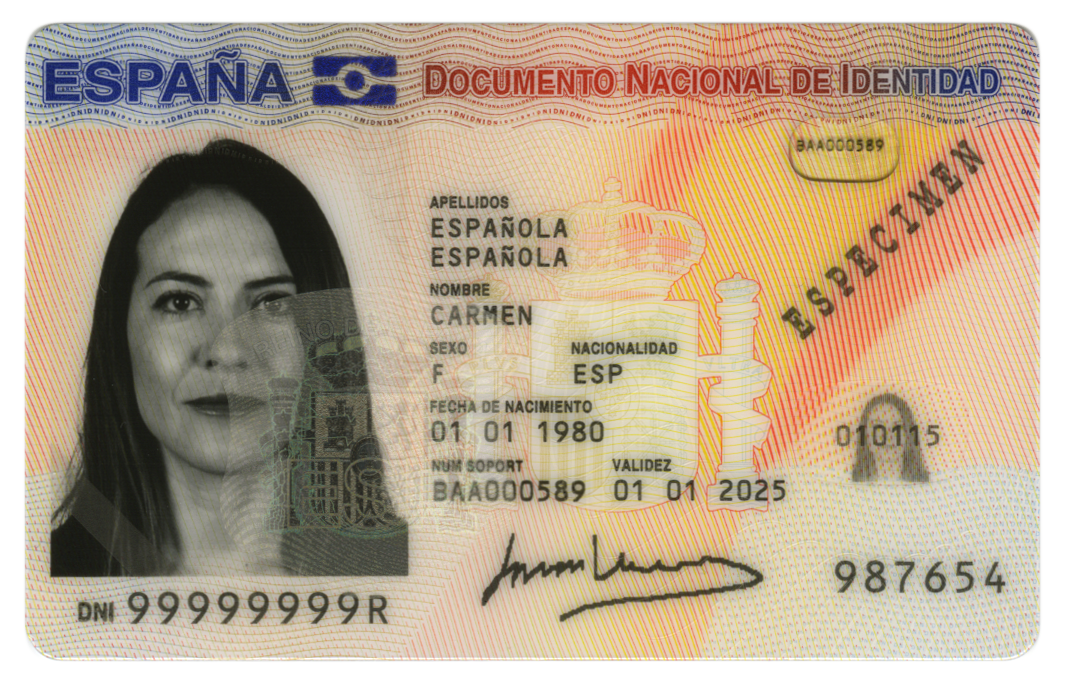
\includegraphics[width=66mm]{images/anverso_3.png}}
	\caption{Comparación del DNI-e con el DNI 3.0} 
\end{figure}

La principal novedad del DNI 3.0 a su antecesor es la presencia de un chip con interfaz dual que permite la conexión mediante hardware, pero tambíen de forma inalámbrica a través de la tecnología NFC (\textit{Near Field Comunication}). No obstante tiene algunas ventajas como:

\begin{itemize}
	\item Incorpora la tecnología de interfaz dual (NFC): gracias a un campo electromagnético entre el dispositivo y la tarjeta se puede intercambiar información. Lo que hace que no tenga la necesidad de utilizar un lector de tarjetas convencional.
	\item Para utilizarlo, solamente es necesario un dispositivo móvil con tecnología NFC y la app del servicio al que nos queremos conectar.
\end{itemize}

Por tanto, el ciudadano no tendrá que descargarse ningún certificado o driver, sino que la conexión se iniciará simplemente con acercar el DNI 3.0 a la antena NFC del dispositivo.

\begin{figure}[H]
	\centering
	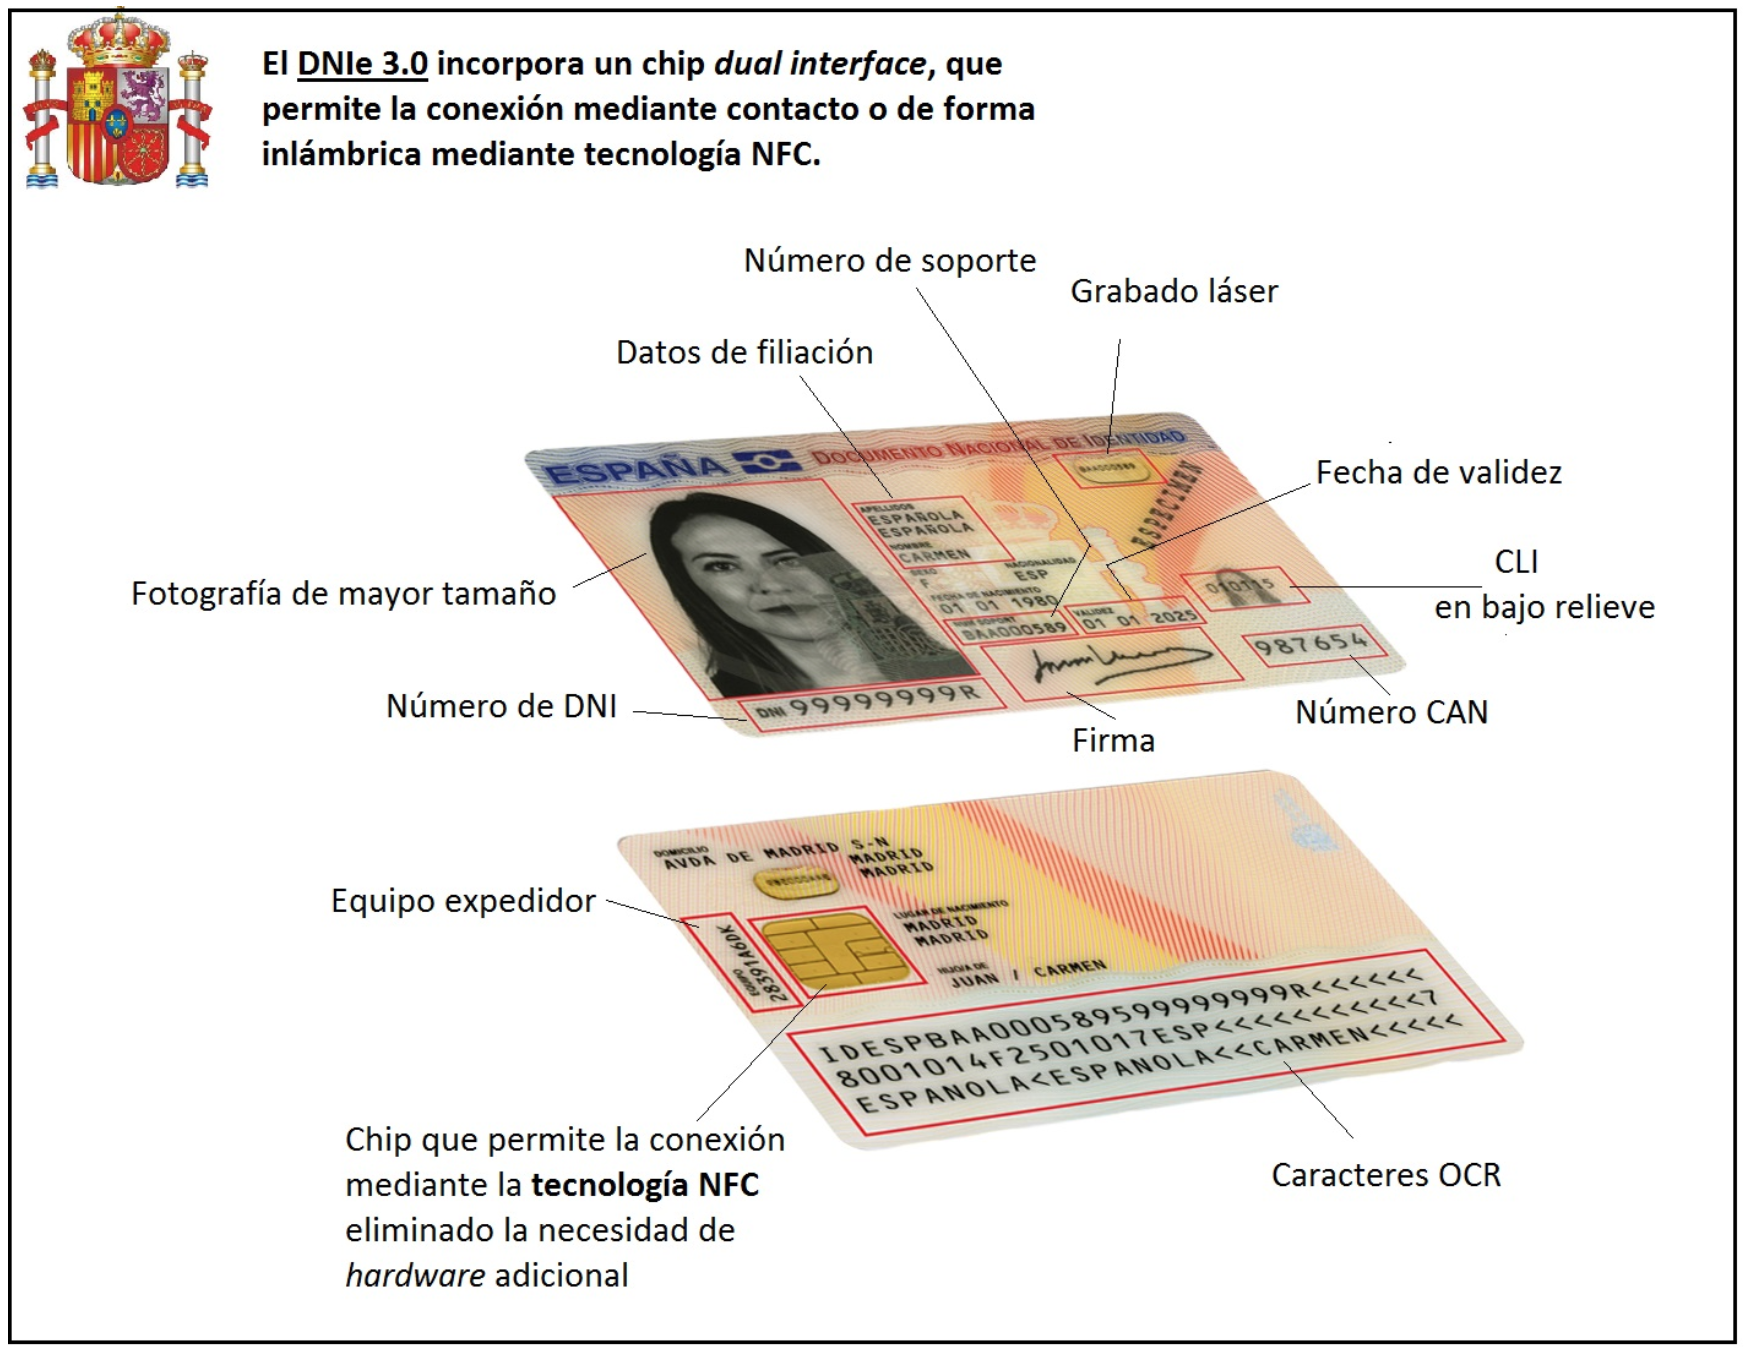
\includegraphics[width=130mm]{images/dni3}
	\caption{Descripción DNI 3.0} 
\end{figure}



\begin{figure}[H]
	\centering
	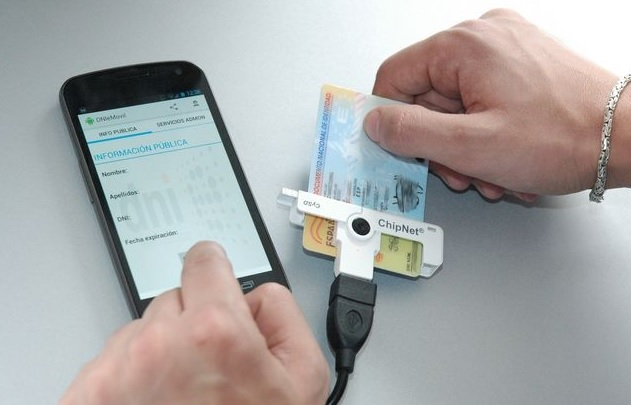
\includegraphics[width=110mm]{images/dni-electronico}
	\caption{DNI-e y lector de tarjetas} 
\end{figure}


\vspace{0.2cm}
\section{Firma electrónica}


El rápido avance tecnológico de la sociedad de hoy en día ha provocado un cambio en muchos hábitos de vida. Muchas acciones que antes se hacían de forma física o telefónicamente (declaración de la renta, compra, transacciones bancarias...), actualmente se pueden hacer sentados delante de un ordenador. 

Como comentamos el inicio del trabajo, cuando firmamos un documento, estamos dando conformidad a lo que está escrito en ese documento. Por lo que una modificación sería detectable, pues dejaría huellas físicas. Además, al disponer la firma de unas características propias de la persona que firma, nadie podría suplantar esa firma. Podemos transpasar esta idea a los documentos digitales. En este caso, el añadido debería ser un conjunto de bits, y si éstos son los mismos para todos los documentos firmados por un usuario, cualquiera podría firmar un documento por él, cosa que no debería de producirse. Por tanto, la firma digital debe ser un añadido al documento que sólo pueda ser realizado por el firmante, pero que además deba variar con el mensaje, es decir, dependa del documento, en cuestión.

\subsection{¿Qué es la firma electrónica?}

\begin{center}\textbf{Una firma electrónica es un concepto legal.}\end{center}

La \textbf{firma electrónica} es el conjunto de datos en forma electrónica, consignados junto a otros o asociados con ellos, que pueden ser utilizados como medio de identificación del firmante. La firma electrónica reconocida tiene el mismo valor que la firma tradicional. Algunas características que debe satisfacer son:

\begin{itemize}
	\item \textbf{Únicas}: sólo puede ser generada por el firmante. 
	\item \textbf{Verificables}: debe ser fácilmente verificable, tanto por receptor como por jueces.
	\item \textbf{No repudiables}: el firmante no puede negar haber realizado la firma. 
	\item \textbf{Viables}: la firma debe ser fácil de realizar.
\end{itemize}	


\subsection{¿A qué nos referimos con firma digital?}

\begin{center}\textbf{Todas las firmas digitales son electrónicas, pero no todas las firmas electrónicas son digitales}\end{center}


En otro orden de ideas, debemos destacar que la \textbf{firma digital} no es sinónimo de firma electrónica, ya que ésta es un método criptográfico que asocia la identidad de una persona o de un equipo informático al mensaje o documento, es decir, se refiere a la tecnología de cifrado/descifrado en la que se basan algunas firmas electrónicas. Por tanto, la firma electrónica pasa a ser un concepto más amplio que el de firma digital. Mientras que la firma digital hace referencia a una serie de métodos criptográficos, el concepto de firma electrónica es de naturaleza fundamentalmente legal, ya que confiere a la firma un marco normativo que le otorga validez jurídica. 

%La firma digital utiliza una combinación de la llave privada del firmante junto con una huella digital (resumen del documento a firmar). Al depender de estos dos factores, solo puede firmar aquella persona dueña del certificado y garantiza que el texto no ha sido manipulado o modificado por terceros.

La firma digital de un documento es el resultado de aplicar cierto algoritmo matemático, denominado función hash, a su contenido y, seguidamente, aplicar el algoritmo de firma (en el que se emplea una clave privada) al resultado de la operación anterior, generando la firma electrónica. La función hash es un algoritmo matemático que permite calcular un valor resumen de los datos a ser firmados digitalmente. Funciona en una sola dirección, no es posible, a partir del valor resumen, calcular los datos originales. Cuando la entrada es un documento, el resultado de la función es un número que identifica inequívocamente al texto. Si se adjunta este número al texto, el destinatario puede aplicar de nuevo la función y comprobar su resultado con el que ha recibido. 

\begin{figure}[H]
	\centering
	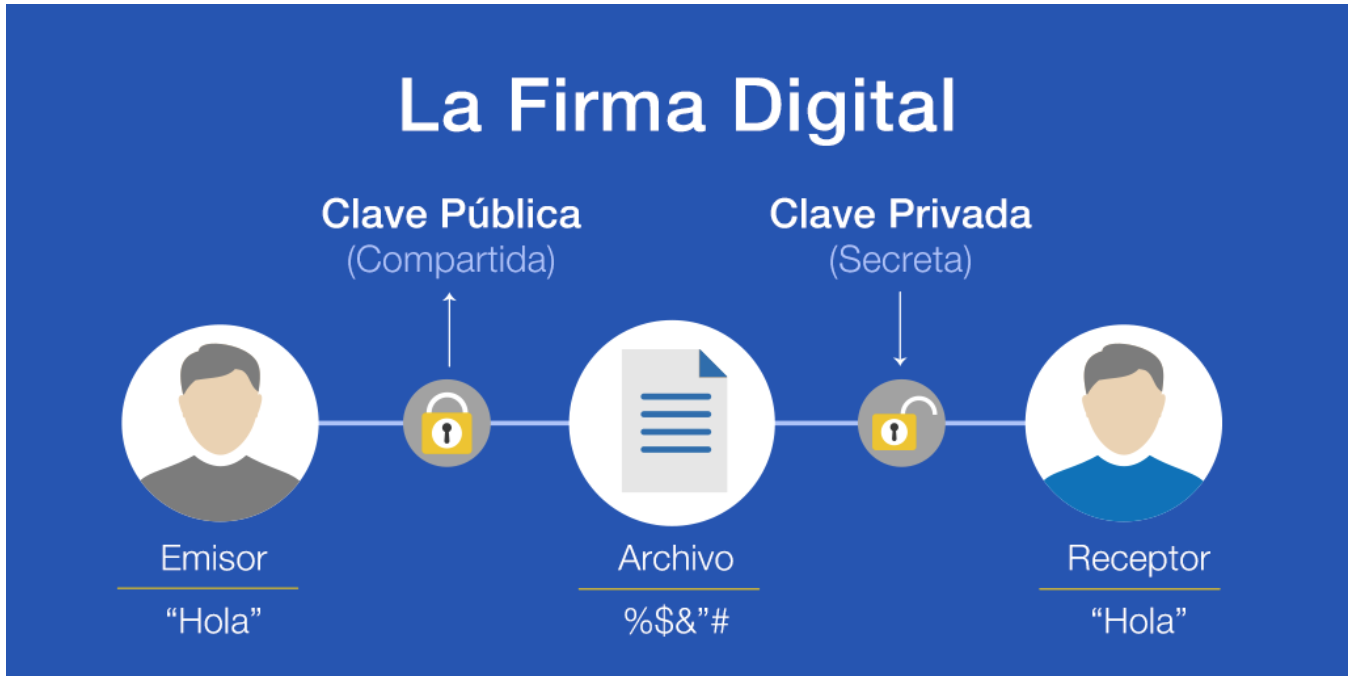
\includegraphics[width=95mm]{images/firma}
	\caption{Firma digital} 
\end{figure}

Por tanto, la firma digital también es legal, pero no tiene naturaleza jurídica, en el sentido de que su objetivo no es dar fe de un acto de voluntad por parte del firmante, sino tan sólo encriptar los datos de un documento para conferirle mayor seguridad. La firma electrónica es una expresión genérica y mucho más amplia relativa a los datos electrónicos y la firma digital es la firma con criptografía basada en clave pública.


\begin{figure}[H]
	\centering
	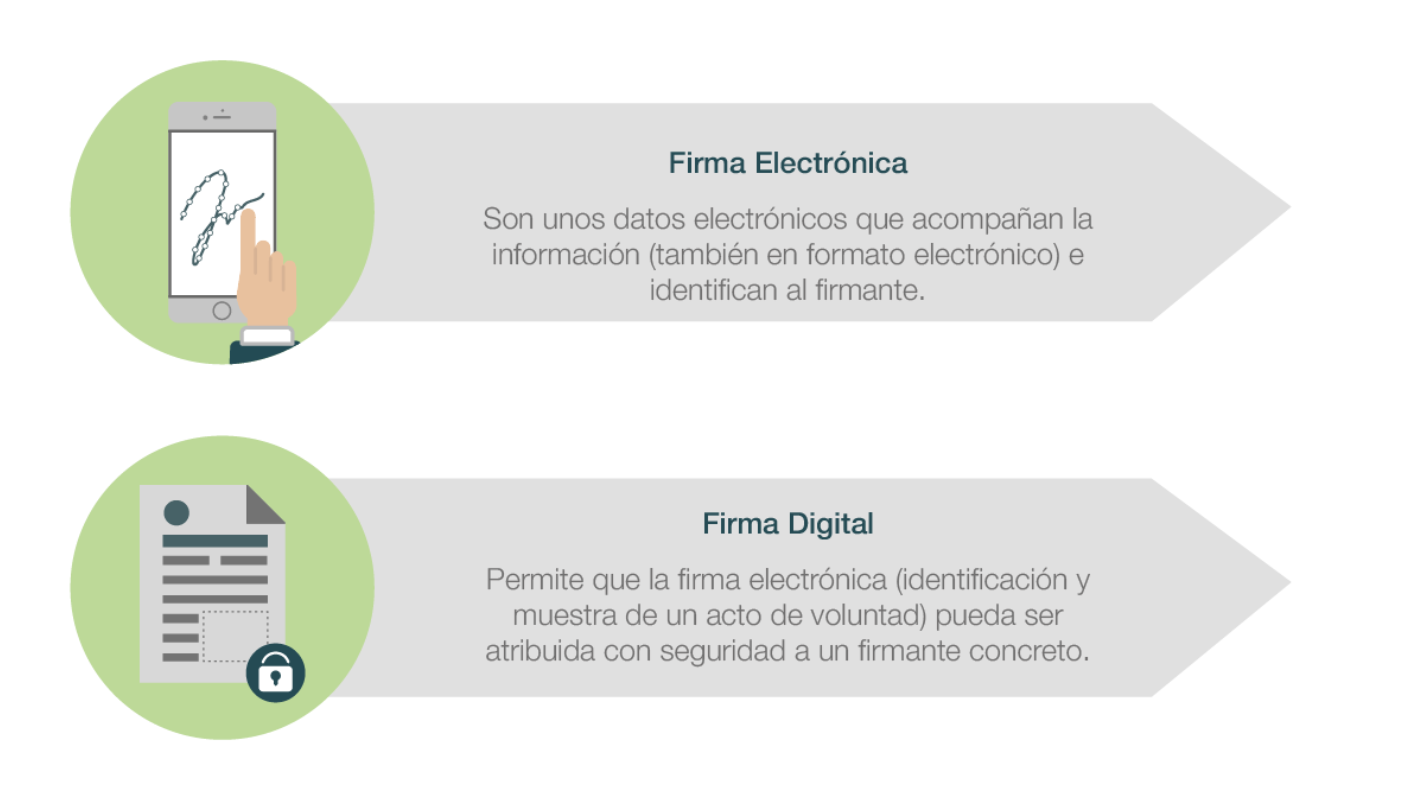
\includegraphics[width=110mm]{images/fd}
	\caption{Firma digital} 
\end{figure}

En resumen, la firma digital es una parte fundamental de la firma electrónica avanzada pero no de la firma electrónica simple (PIN ingresado en un cajero automático del banco o hacer clic en la casilla 'aceptar"). Ya que este tipo de firma electrónica no permite atribuir la firma a un firmante en concreto, por lo que no reúne las características de la firma digital.


\begin{figure}[H]
	\centering
	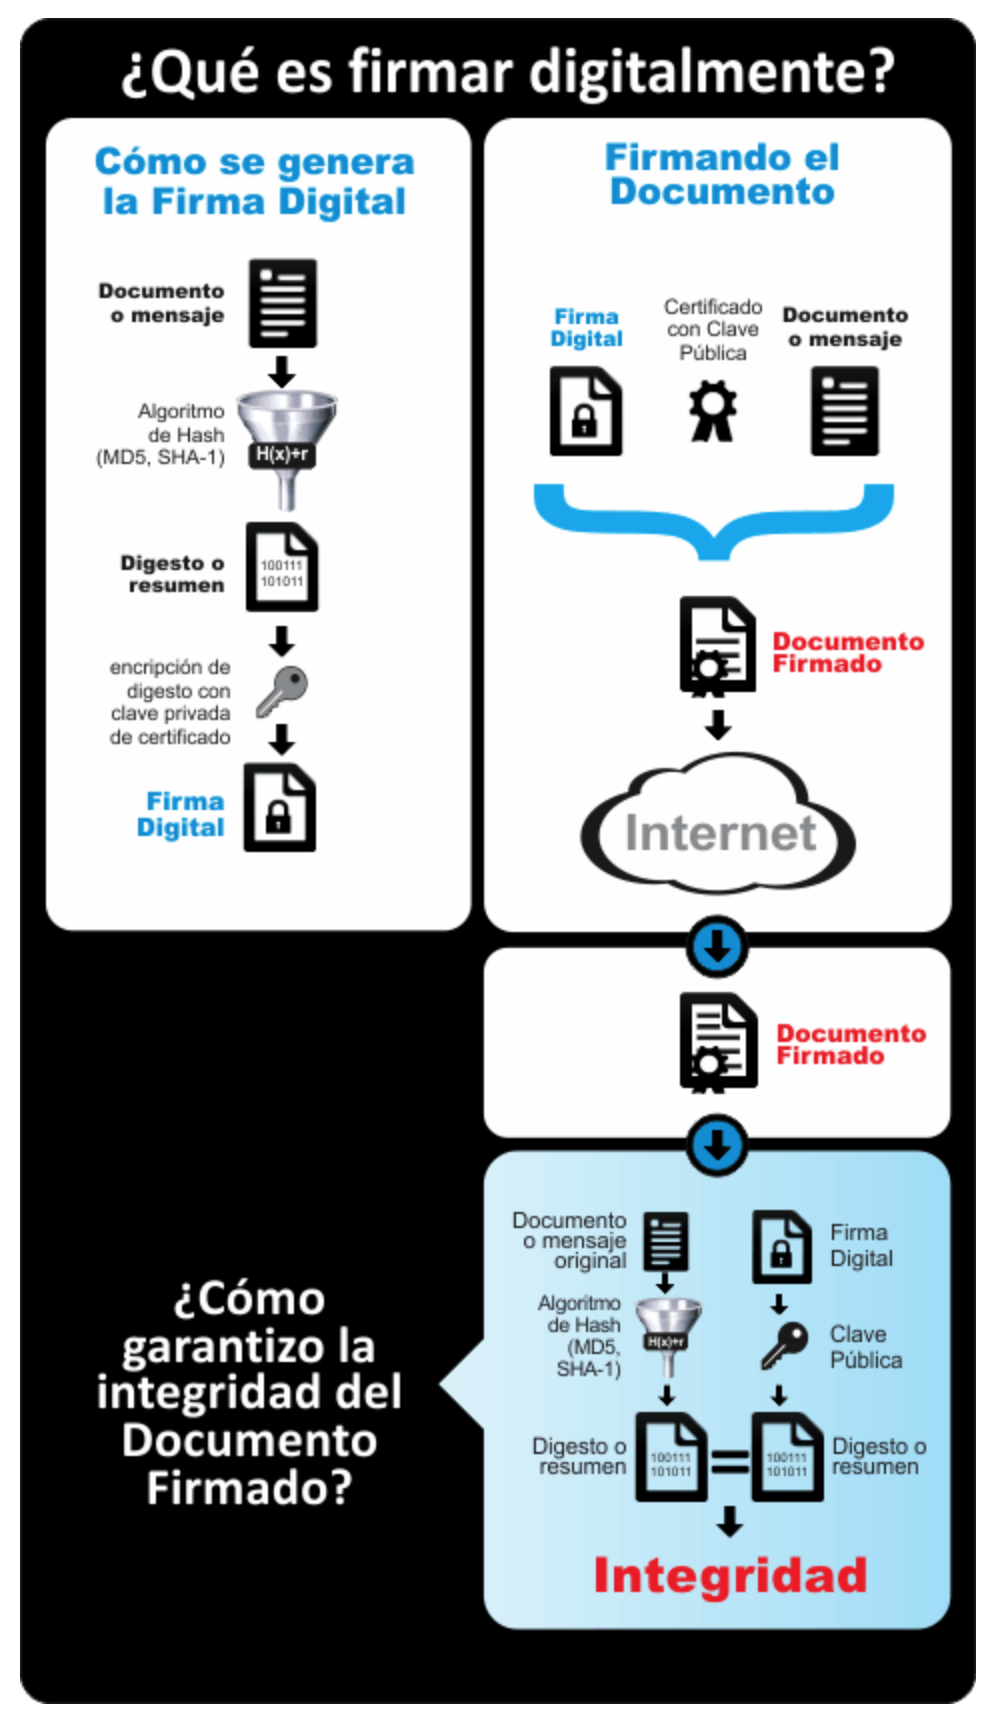
\includegraphics[width=90mm]{images/digital.png}
	\caption{Funcionamiento de la firma digital} 
\end{figure}






%Funcionamiento de la firma digital [imagen]


%Comprobación de firma [imagen]



\subsubsection{Ejemplo de implementación firma digital}

En este punto se va \textbf{implementar un sistema de firma digital y verificación de la firma} con RSA. Para ello se deben de realizar tres tareas: \textbf{generación de claves}, \textbf{generación de firma} y \textbf{verificación de firma}.

\begin{center}\textbf{El código completo se puede encontrar en mi Github: \url{https://github.com/Gecofer/MII_ASS_1819}}\end{center}

\underline{\textbf{1. Generación de claves}}

Para la generación de la clave, nos basamos en la función que implementa un \textbf{RSA}. El sistema criptográfico con clave pública RSA es un algoritmo asimétrico cifrado de bloques, que utiliza una clave pública, la cual se distribuye, y otra privada, la cual es guardada en secreto por su propietario. Los mensajes enviados usando el algoritmo RSA se representan mediante números y el funcionamiento se basa en el producto de dos números primos grandes (mayores que $10^{100}$) elegidos al azar para conformar la clave de descifrado\footnote{https://seguinfo.wordpress.com/2007/09/14/\%C2\%BFque-es-rsa/}. El algoritmo RSA funciona de la siguiente manera:

\begin{enumerate}
	\item Para elegir la pareja de claves, lo primero que necesitamos es elegir dos primos grandes $p$ y $q$, y calcular su producto $n = p \cdot q$.
	
	\item Ahora se elige un entero $e$ tal que $mcd(e,\phi(n)) = 1$. Recordemos que $\phi(n) = (p-1)\cdot(q-1)$. Ambos valores, $(n, e)$ constituyen la clave pública del criptosistema. El número $n$ se conoce como módulo del Criptosistema.
	
	\item La clave privada es un entero $d$ tal que $d \cdot e = 1 (mod\ {\phi(n)})$.
\end{enumerate}

Dichas claves de RSA, las guardaremos en un fichero. Por tanto, la función creada tiene como salida: $e,n$ que será clave pública y $d$ que será la clave privada.

\begin{figure}[H]
	\centering
	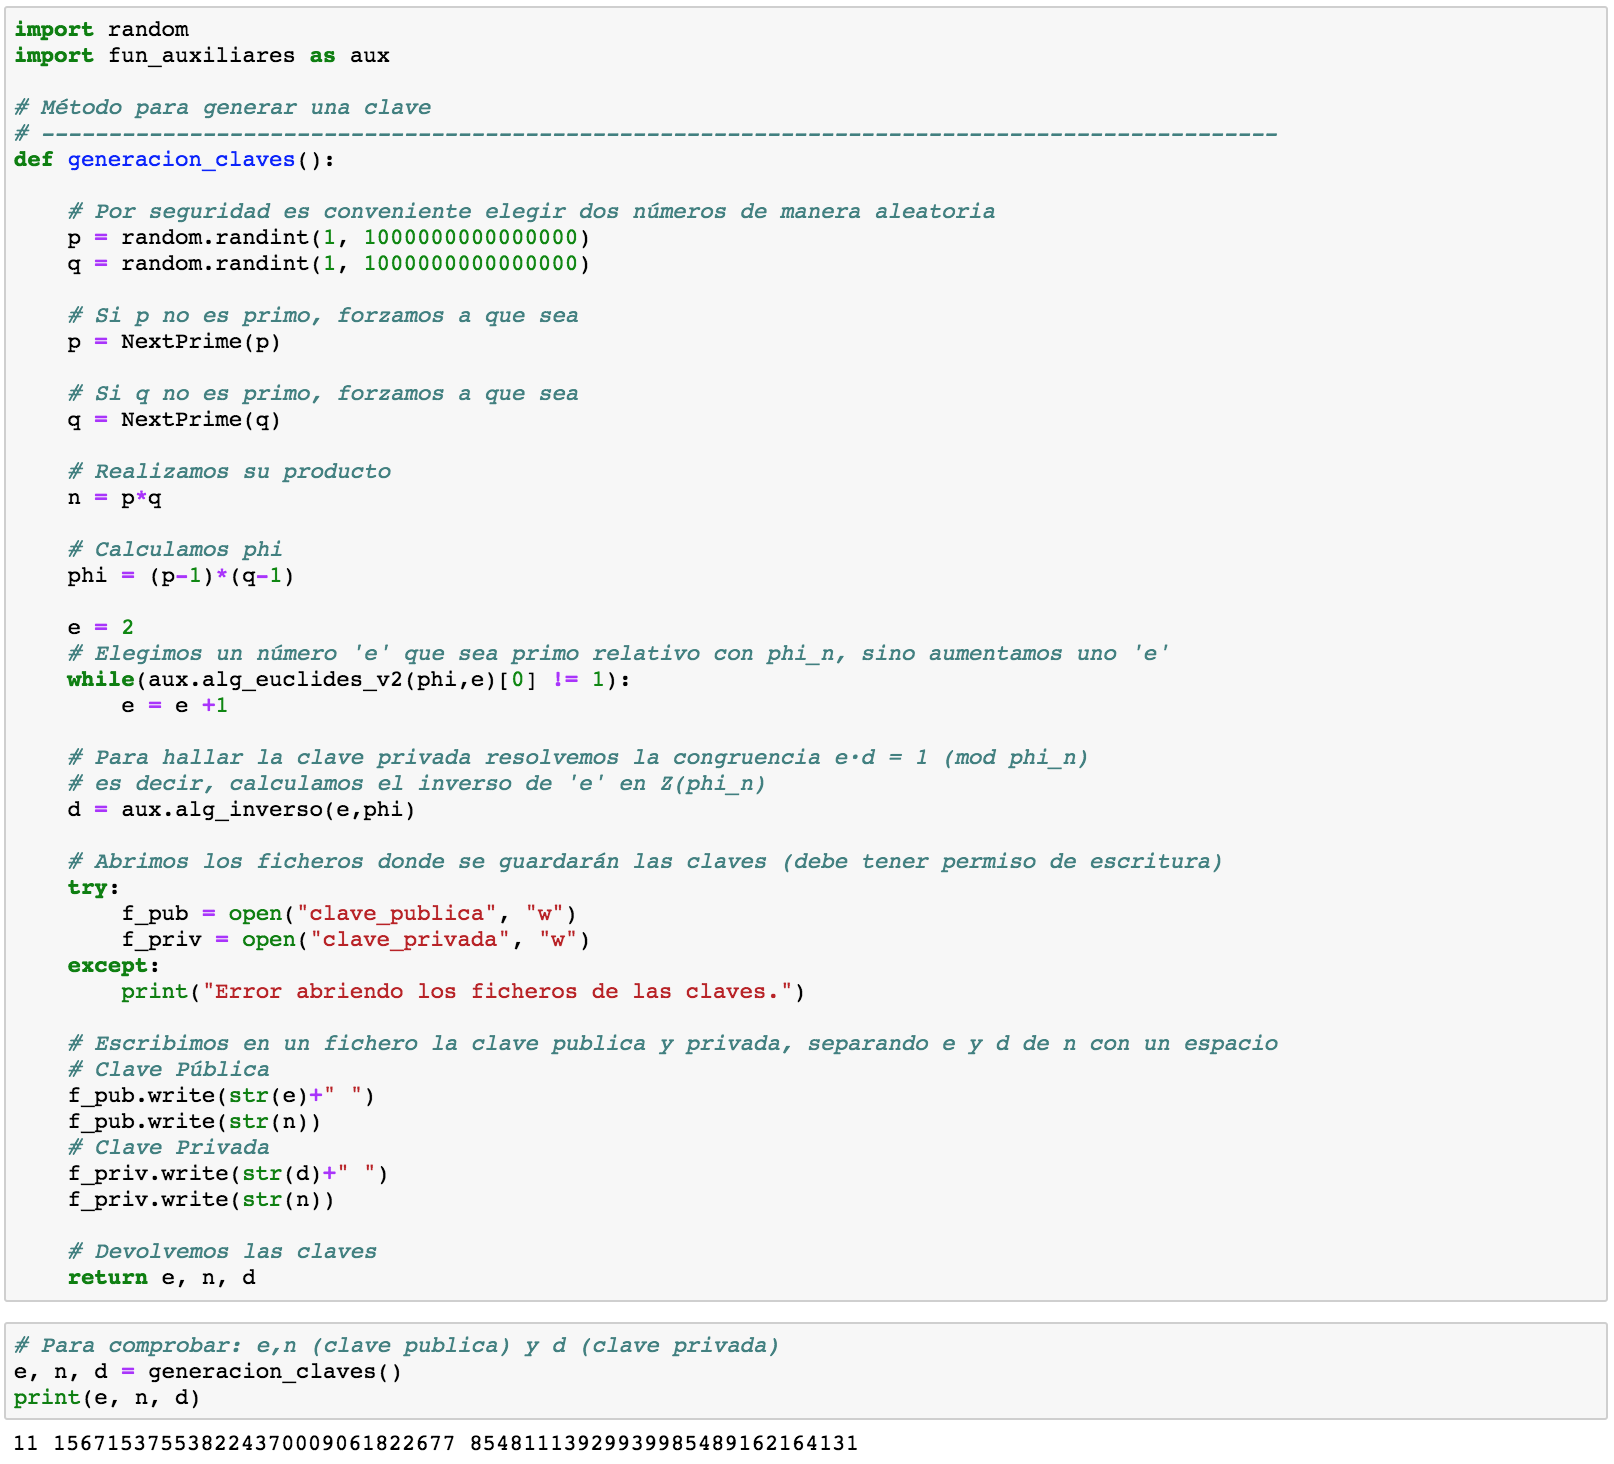
\includegraphics[width=145mm]{images/1}
	\caption{Función para generar las claves} 
\end{figure}

\newpage

\underline{\textbf{2. Generación de firma}}

Para la \textbf{generación de la firma}, se le introducirá un mensaje a cifrar (fichero) y el fichero con la clave (privada), y deberá generar una firma, que se guardará en un fichero de texto. En este caso, el mensaje será \textit{Hola}, y la clave privada la hemos obtenido en el apartado anterior. Puesto que lo que realmente se firma no es el mensaje, sino un resumen del mensaje, hay que generar un resumen de dicho mensaje. Para esto emplearemos la función \textbf{SHA1} (se pueden añadir otras funciones resumen). Dicha función hash es un algoritmo matemático que permite calcular un valor resumen de los datos a ser firmados digitalmente.

\begin{figure}[H]
	\centering
	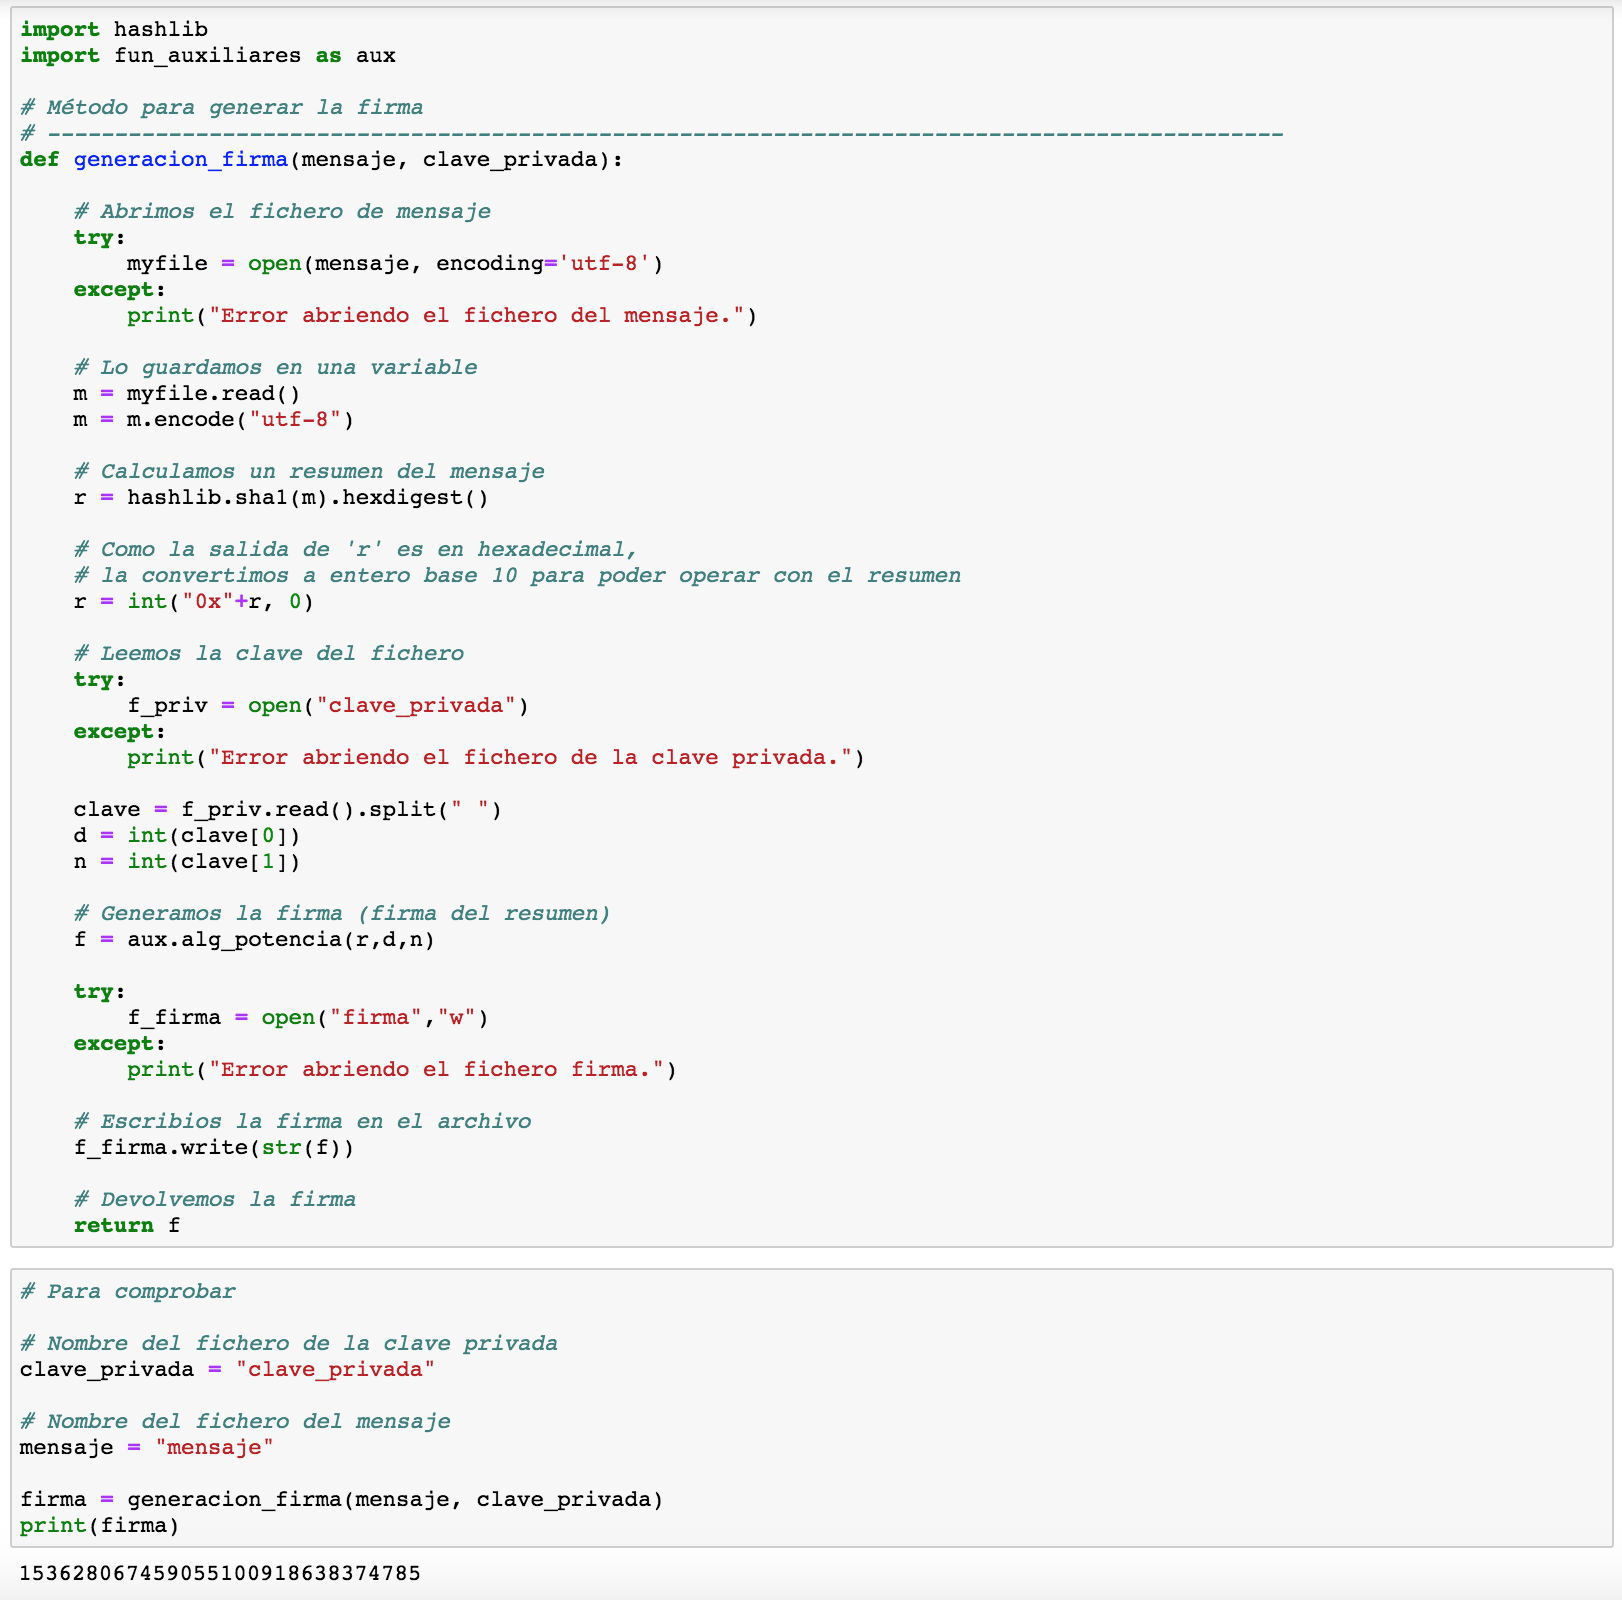
\includegraphics[width=145mm]{images/2}
	\caption{Función para generar la firma} 
\end{figure}

Para la función SHA1, usaremos la librería de Python \texttt{hashlib}, que ya implementa esa función. Para generar una firma, solo nos bastaría hacer $fir(r) = r^d (mod\ n)$. Por tanto, el mensaje firmado sería el par $(r, fir(r))$.

\begin{itemize}
	\item \textbf{Entrada} de la función: 
	\begin{enumerate}
		\item $mensaje$: nombre del fichero del mensaje a firmar en string
		\item $clave-privada$: nombre del fichero de la clave privada en string (contiene $d$ y $n$)
	\end{enumerate}
	
	\item \textbf{Salida} de la función: 
	\begin{enumerate}
		\item $f$: firma del resumen del mensaje
	\end{enumerate}
\end{itemize}	

\underline{\textbf{3. Verificación de la firma}}

Para la \textbf{verificación de la firma}, se introduce el mensaje (fichero) que se ha firmado, un fichero con la firma (con el mismo formato que el generado en el apartado anterior) y un fichero con la clave (pública). Y deberá responder si la firma es o no válida. Para comprobar si la firma es válida, habría que hacer si $r = fir(r)^e (mod\ n)$.

\begin{figure}[H]
	\centering
	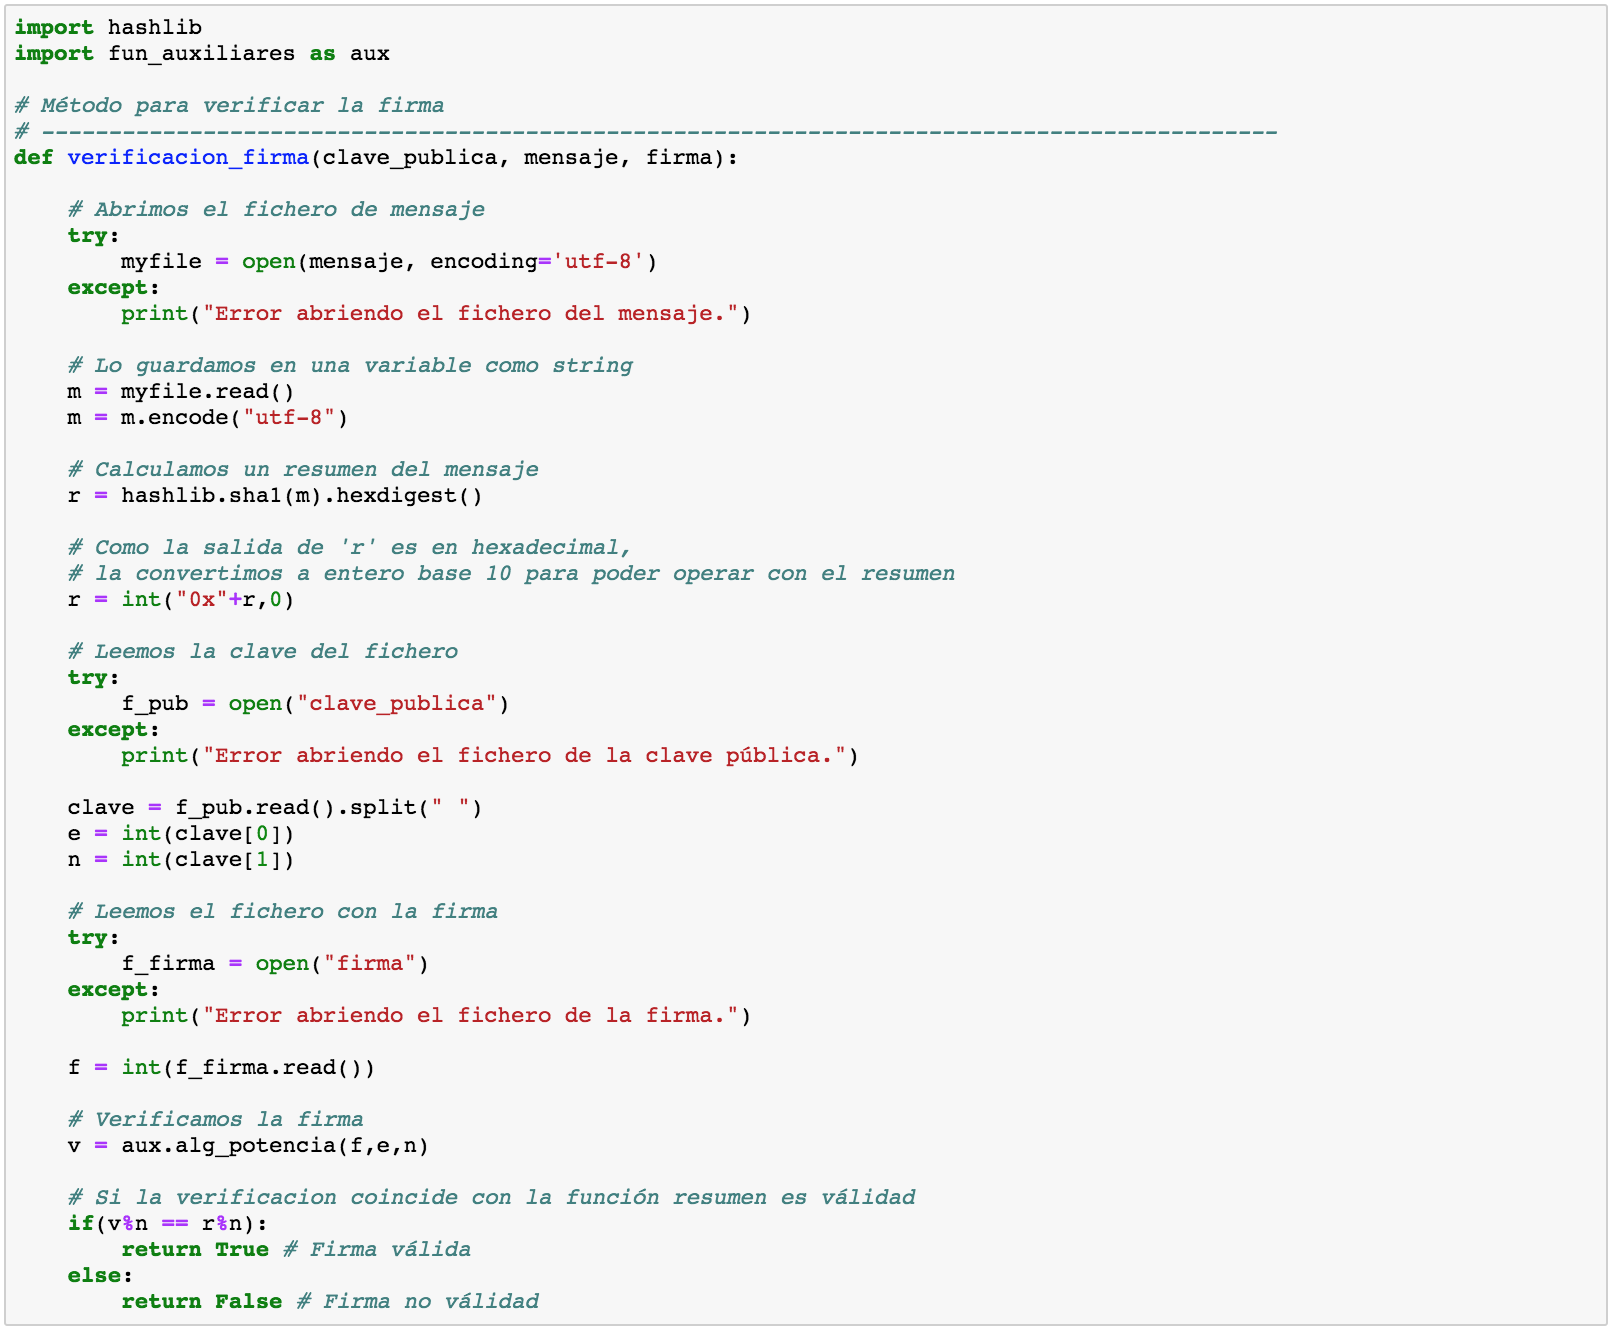
\includegraphics[width=145mm]{images/3}
	\caption{Función para verificar la firma} 
\end{figure}

\begin{itemize}
	\item \textbf{Entrada} de la función: 
		\begin{enumerate}
			\item $clave-publica$: nombre del fichero de la clave pública en string ($e$ y $n$)
			\item $mensaje$: nombre del fichero del mensaje a verificar en string
			\item $firma$: nombre del fichero de firma en string
		\end{enumerate}	
	
	\item \textbf{Salida} de la función: 
		\begin{enumerate}
			\item $True$: si la firma es correcta
			\item $False$: si la firma no es correcta
 		\end{enumerate}	
\end{itemize}				



\begin{figure}[H]
	\centering
	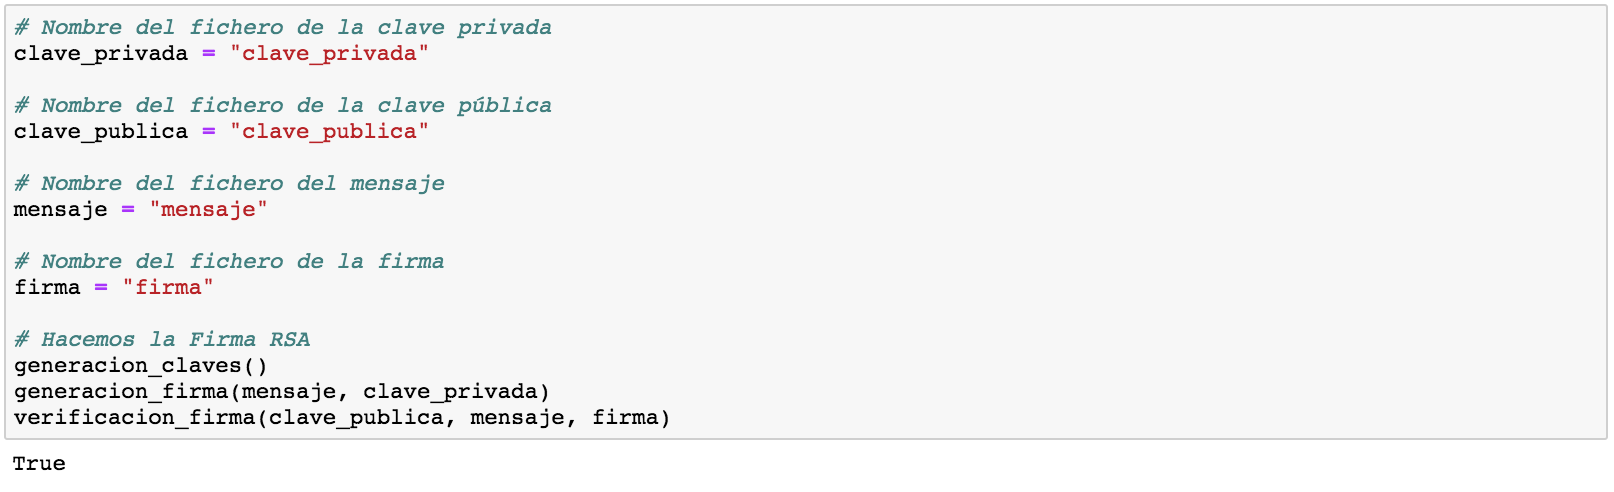
\includegraphics[width=145mm]{images/4}
	\caption{Comprobación del sistema y verificación de la firma digital} 
\end{figure}

Con esto acabamos de comprobar la verificación de la firma, para un mensaje \textit{Hola}. Por tanto, si queremos comprobar que la verificación funciona, solo hace falta editar el fichero de firma y realizar de nuevo la verificación, con lo que obtendremos un valor $False$.

% [VER APUNTES DE CRIPTOGRAFÍA]


% https://seguinfo.wordpress.com/2007/09/14/%C2%BFque-es-rsa/


\vspace{0.2cm}
\section{Conclusiones}


Después de analizar los distintos tipos de certificados y ver sus ventajas e inconvenientes, se ha de destacar la flexibilidad de la que dota el certificado software emitido por la FMNT. Pero es decisión del usuario, elegir la opción que mejor se adecue a sus necesidades. Sin embargo, actualmente ambos tipos de certificados se complementan, ya que prácticamente todas las webs que disponen de certificado digital mediante software, también tienen la posibilidad de usar el DNI electrónico. Además, la necesidad de evolución en el mundo tecnológico supuso dar el salto del DNI electrónico al DNI 3.0, el cuál permite una mayor usabilidad del mismo al permitir el acceso y autenticación con él a través de la tecnología NFC y no de la necesidad de usar un lector de tarjetas, lo que complicaba su uso mediante la instalación de drivers y adquisición del lector. 

Por otro lado, cabe destacar que la funcionalidad del DNI electrónico, se basa fuertemente en la firma electrónica, la cual permite la identificación del firmante. Además, es importante señalar que esta firma tiene el mismo valor que la firma tradicional, cosa que con el certificado software no ocurre.

No obstante, las nuevas tecnologías del futuro evolucionarán hacia tecnologías más seguras y hacia la unificación de un único medio digital para la realización de dicha autenticación e identificación, pero aún queda mucho por recorrer. 




%Ejemplo del certificado digital con el ordenador

%Ejemplo del DNI electronico con el móvil


%¿Existe diferencia entre un certificado digital y electrónico?

%¿Puede alguien hacerse pasar por mí con el certificado digital?

%¿Qué es mejor un certificado digital  o DNIe?

% https://www.adminfacil.es/dni-electronico-vs-certificado-digital/


%¿Es posible digitalizar un DNI que no sea electrgonico?


%https://sede.seg-social.gob.es/wps/portal/sede/sede/Inicio/CertificadosDigitales/dni%20electronico/03dni%20electronico/!ut/p/z1/jZDNqsIwEIVfxU2XdqZGpHVX9HKvPwVFSms2UntjGmiTkkYLPr0B3SjaOrs5fGc4Z4BCClRmF8EzI5TMSrvv6eRAvMnYC9Bb_-LiB8M4WsUB2RKcjyDpBAIE-o0fP0zY61_2AbbBSEeziAOtM1MMhTwpSP-lGLCS5UYrKXIrIHmVEqCdtwOvD8AH0NHOxuelOt4_Hcoj8W1OzU5MM-2etZULY-pm6qCDbdu6XCleMjdXlYPvLIVqDKTPJOxYA3UVp9f1H4pNlfjGD2_X2lKF/dz/d5/L2dBISEvZ0FBIS9nQSEh/

%https://www.sede.fnmt.gob.es/certificados



% \begin{figure}[H]
% \centering
% \subfigure[Modelo a realizar]{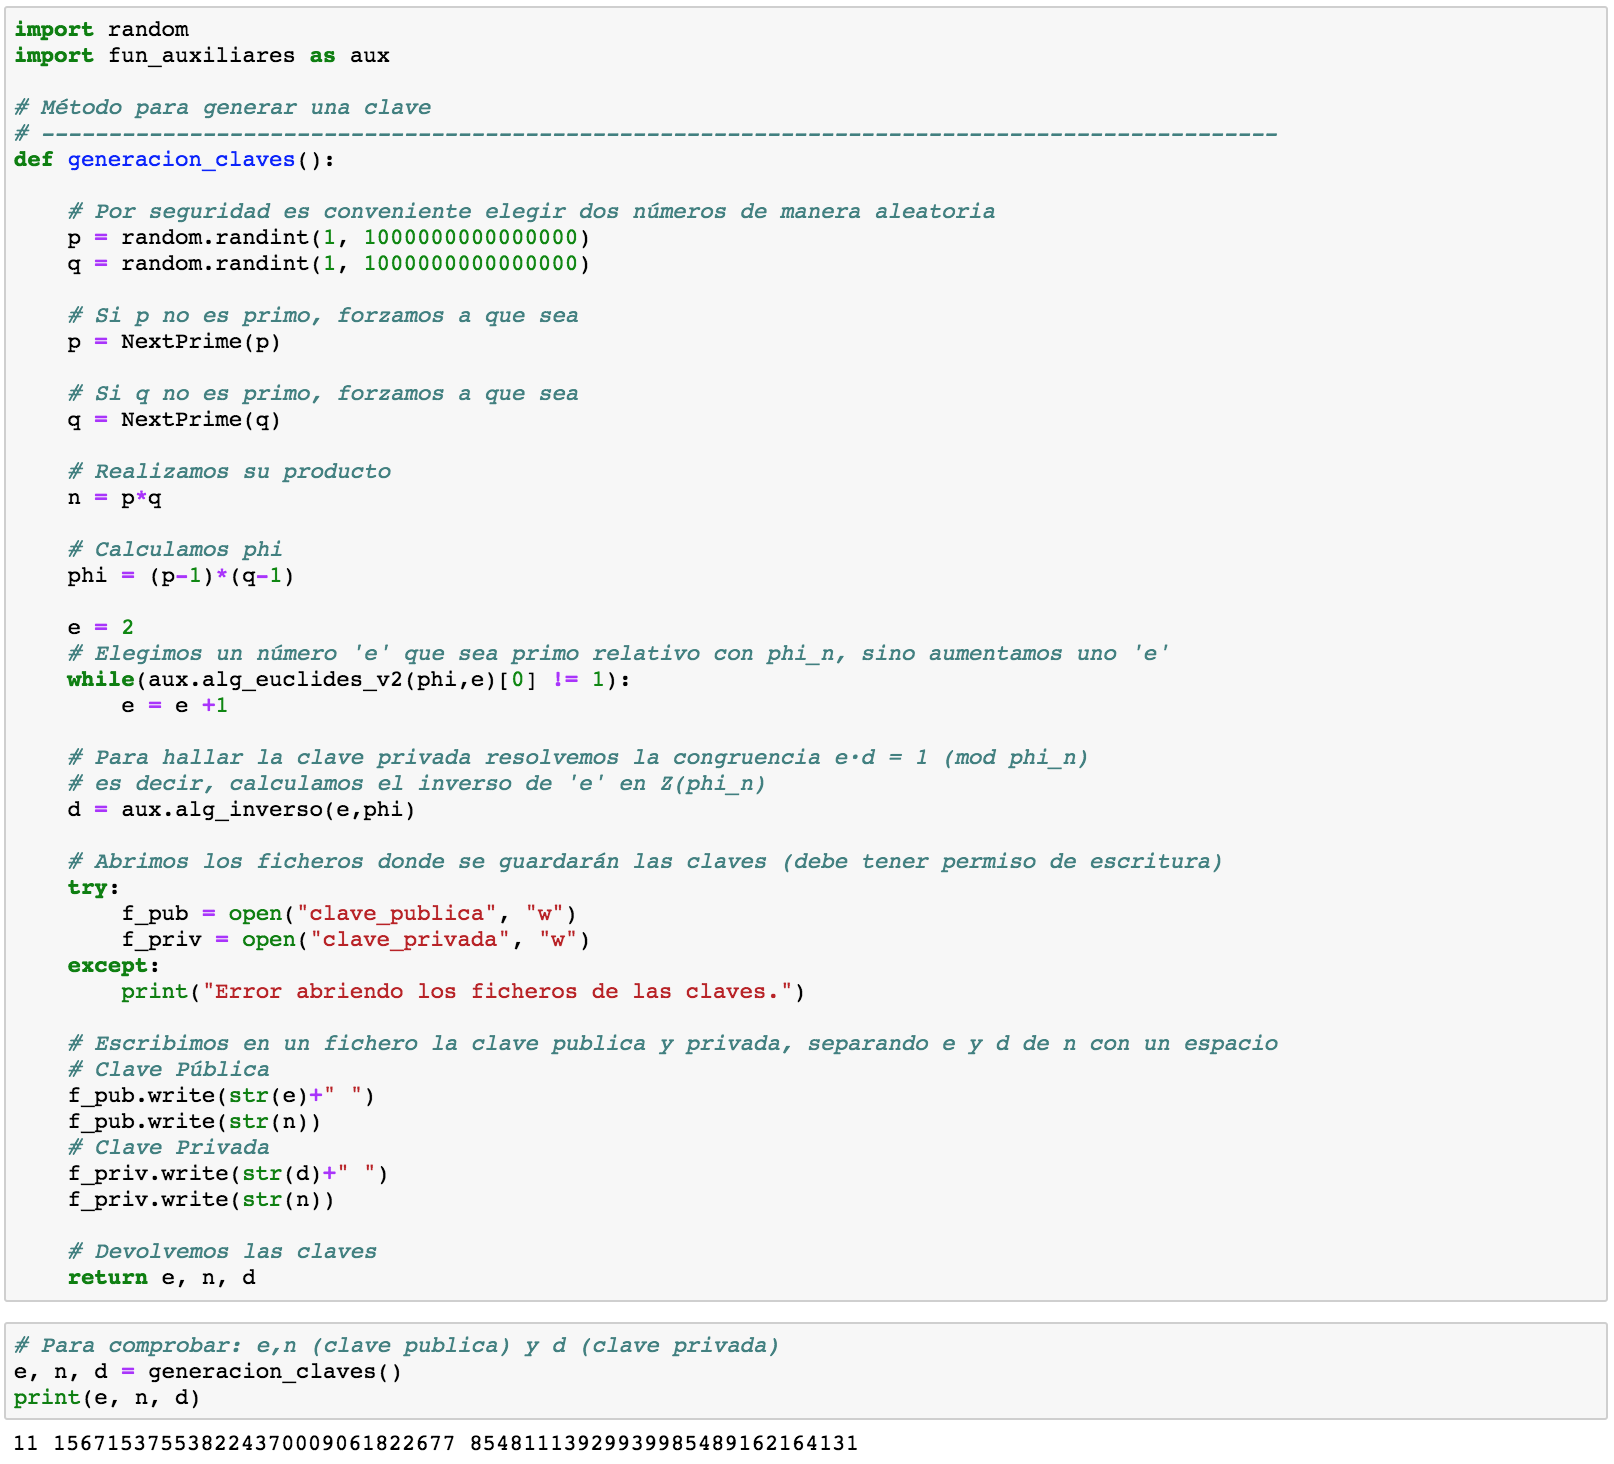
\includegraphics[width=65mm]{images/1}}
% \subfigure[Modelo actual]{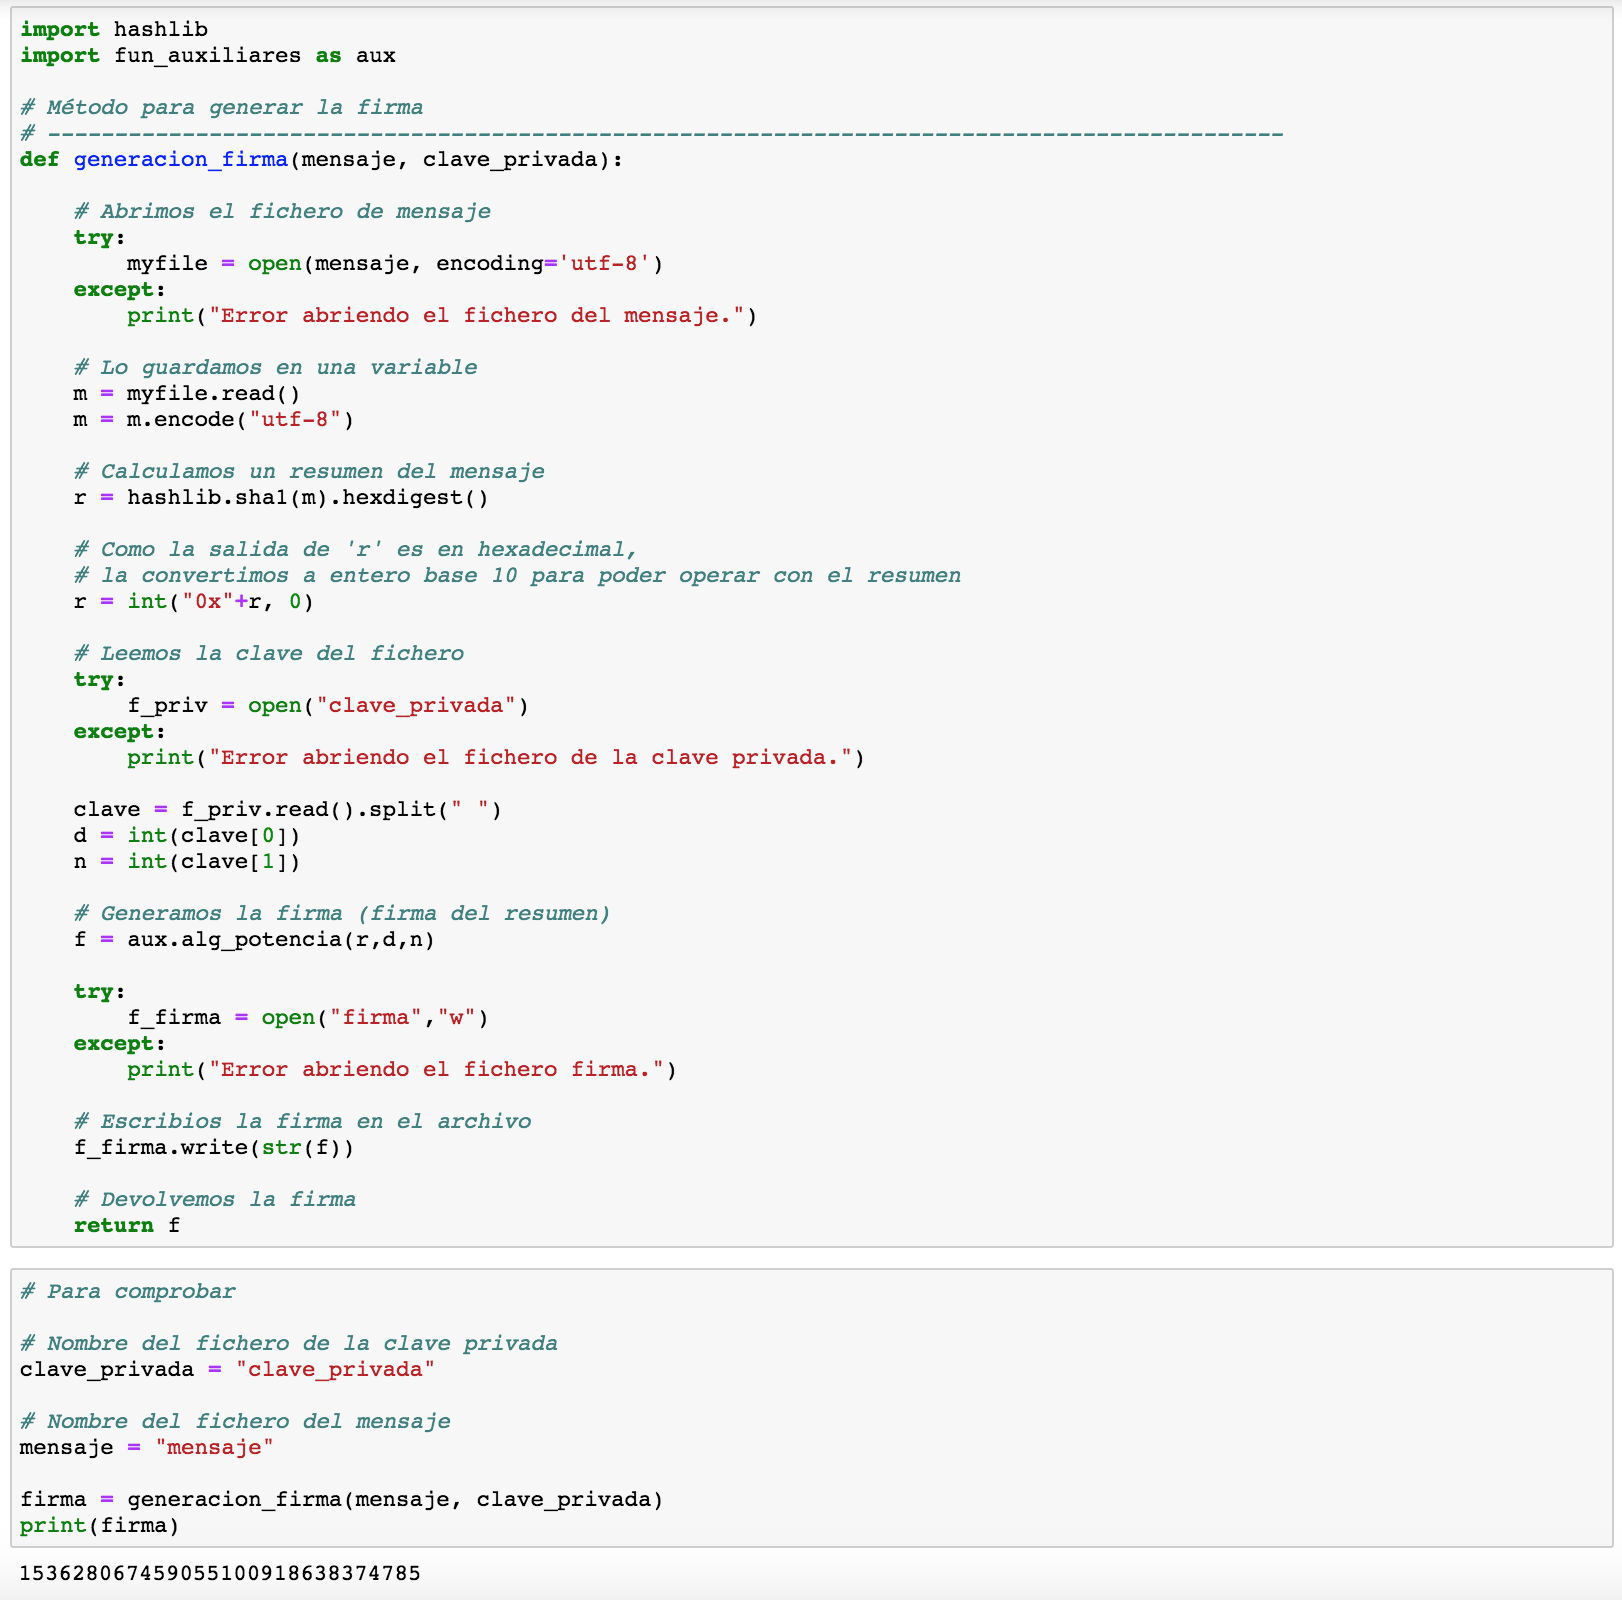
\includegraphics[width=76mm]{images/2}}
% \caption{Modelo} \label{tema}
% \end{figure}

%%%%%%%%%%%%%%%%%%%%%%%%%%%%% Referencias %%%%%%%%%%%%%%%%%%%%%%%%%%%%%
\newpage
%\section{Referencias}
\addcontentsline{toc}{section}{Referencias}
\nocite{*}
\printbibliography
%\bibliographystyle{unsrt}
%\bibliography{references}

%\bibliographystyle{IEEEtran}
%\bibliography{references}
%\nocite{*}
%\printbibliography[
%heading=bibintoc,
%title={Referencias}
%] %Prints the entire bibliography with the titel "Whole bibliography"


%%%%%%%%%%%%%%%%%%%%%%%%%%%%%%%%%%%%%%%%%%%%%%%%%%%%%%%%%%%%%%%%%%%%%%%

\end{document}


